%%% Pulsars and supernovae notes.

\documentclass{momento}

\usepackage{tabularx}
\usepackage{danielphysics}
\usepackage{tensor}
\usepackage{multirow, mhchem}

\title{Pulsars and Supernovae}
\author{Daniel Williams}


\newcommand*\circled[1]{\tikz[baseline=(char.base)]{
            \node[shape=circle,fill=white,draw,inner sep=2pt] (char) {#1};}}

\providecommand{\Lag}{\mathcal{L}} %The Lagrangian
\providecommand{\Op}[1]{\mathrm{\hat{#1}}}  %A Quantum mechanical operator
\providecommand{\Lap}{\bigtriangleup}

\begin{document}
\frontmatter
{
\thispagestyle{empty}

\begin{tikzpicture}[remember picture,overlay]
  \fill[fill=Purple] (current page.south west) rectangle (current page.north east);
  %\fill[fill=white, yshift=-10cm]  (current page.north east) rectangle (current page.north west);
  \def\nbrcircles {377}
  \def\outerradius {30mm}
  \def\deviation {.9}
  \def\fudge {.62}

  \newcounter{cumulArea}
  \setcounter{cumulArea}{0}

  \pgfmathsetmacro {\goldenRatio} {(1+sqrt(5))}
  \pgfmathsetmacro {\meanArea} {pow(\outerradius * 10 / \nbrcircles, 2) * pi}
  \pgfmathsetmacro {\minArea} {\meanArea * (1 - \deviation)}
  \pgfmathsetmacro {\midArea} {\meanArea * (1 + \deviation) - \minArea}

  \foreach \b in {0,...,\nbrcircles}{
    % mod() must be used in order to calculate the right angle.
    % otherwise, when \b is greater than 28 the angle is greater
    % than 16384 and an error is raised ('Dimension too large').
    % -- thx Tonio for this one.
    \pgfmathsetmacro{\angle}{mod(\goldenRatio * \b, 2) * 180}

    \pgfmathsetmacro{\sratio}{\b / \nbrcircles}
    \pgfmathsetmacro{\smArea}{\minArea + \sratio * \midArea}
    \pgfmathsetmacro{\smRadius}{sqrt(\smArea / pi) / 2 * \fudge}
    \addtocounter{cumulArea}{\smArea};

    \pgfmathparse{sqrt(\value{cumulArea} / pi) / 2}
    \fill[opacity=0.3] (\angle:\pgfmathresult) circle [radius=\smRadius] ;
}  

  \node at (current page.center) [text width=12.5cm, yshift=7cm] 
    {\color{white}\fontsize{72pt}{90pt}\raggedright{ \selectfont\sffamily Pulsars \phantom{pulsar} and Supernovae}};

  \node at (current page.south) [text width= \textwidth, yshift=5cm] 
    {\color{white}\fontsize{32pt}{120pt}\selectfont \sffamily Daniel Williams};

\end{tikzpicture}
}
\newpage
\maketitle

\tableofcontents
\mainmatter
\part{Supernovae}
\label{part:supernovae}


\chapter{Fluid Mechanics}
\label{cha:fluid-mech}


\section{$N$-particle Systems}
\label{sec:n-particle-systems}

Generally a system of $N$ particles can be described by a system of
$6N$ Hamiltonian equations, however, in most systems the size of $N$
is so large that it rapidly becomes impractical to solve such a system
of equations to determine the behaviour of the system, and so at least
one of a number of approaches must be taken to simplify the analysis.

\begin{description}
\item[Test Particles] This is an exact solution for some $M \ll N$
  particles of the system, while the rest are treated as an external
  slowly evolving medium.
\item[Hydrodynamic Descriptions of Plasma] We assume a plasma to be
  continuous at a scale much greater than the mean free path of
  particles within the material.
\item[Classical Kinetics] studies the relationship between motion and
  the forces affecting the motion using statistical methods.
\end{description}

In fluid dynamics the motion of fluids is studied on a macroscopic
scale, with the fluid regarded as a continuous medium. The fluid is
described by macroscopic parameters, such as fluid density, fluid
velocity, and pressure.

\section{Deriving the Hydrodynamic Equations}
\label{sec:deriv-hydr-equat}

\subsection{Conservation of Matter}
\label{sec:conservation-matter}
%\begin{derivation}
  Consider a fluid with a mass density $\rho$, and a volume $V$. The
  mass of the fluid is then
  \begin{equation}
    \label{eq:1}
    m = \int_V \rho \dd{V}
  \end{equation}
\marginpar{
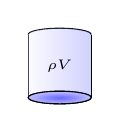
\begin{tikzpicture}[scale=0.4]
    \draw (1,0) arc (180:360:1cm and 0.2cm);
    \draw (1,0) arc (180:0:1cm and 0.2cm);
    \draw (1,2) arc (180:0:1cm and 0.2cm);
	\draw (1,0) -- (1,2); \draw (3,0) -- (3,2);
    \shade[left color=blue!5!white,right color=blue!60!white,opacity=0.3] (1,0) arc (180:360:1cm and -0.2cm) -- (3,0) -- (3,2) arc (180:360:-1cm and -0.2cm) -- (1,2) -- cycle; 
    \shade[draw=black,shading=radial, outer color=blue!25!white,inner color=blue!60!white,opacity=1] (2,0) circle (1cm and 0.2cm);
    \draw (2,1) node {\tiny $\rho V$};
\end{tikzpicture}
}
  Let $\dd{s}$ be a surface element of the volume, then the matter flux
  through that surface is $\rho\ \vec{v}\ \dotproduct \dd{\vec{s}}$, with
  a positive flux representing eflux, and a negative flux
  influx. Assuming there are no sources or sinks inside the volume $V$
  then the total mass of fluid flowing out of the volume $V$ per unit
  time is
  \begin{equation}
    \label{eq:2}
    \dv{m}{t} = \oint_{\partial V} \rho \ \vec{v}\ \dotproduct \dd{\vec{s}} 
    = - \pdv{t} \int_V \rho  \dd{V}
  \end{equation}
\marginpar{
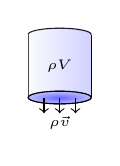
\begin{tikzpicture}[scale=0.4]
    \draw (1,0) arc (180:360:1cm and 0.2cm);
    \draw (1,0) arc (180:0:1cm and 0.2cm);
    \draw (1,2) arc (180:0:1cm and 0.2cm);
	\draw (1,0) -- (1,2); \draw (3,0) -- (3,2);
    \shade[left color=blue!5!white,right color=blue!60!white,opacity=0.3] (1,0) arc (180:360:1cm and -0.2cm) -- (3,0) -- (3,2) arc (180:360:-1cm and -0.2cm) -- (1,2) -- cycle; 
    \shade[draw=black,shading=radial, outer color=blue!25!white,inner color=blue!60!white,opacity=1] (2,0) circle (1cm and 0.2cm);

	\foreach \x in {0.5, 1, ..., 1.75} {
		\draw [<-] (1+\x, -0.5) -- (1+\x, 0);
	}
	\draw (2, -0.8) node {\tiny $\rho\vec{v}$};
	\draw (2,1) node {\tiny $\rho V$};
\end{tikzpicture}
}
  As long as the mass in the volume $V$ is conserved the two expressions
  for the mass, equations (\ref{eq:1}) and (\ref{eq:2}) can be equated.
  \begin{equation}
    \label{eq:3}
    \pdv{t} \int_V \rho \dd{V} = \oint_{\partial V} \rho \ \vec{v}\ \dotproduct \dd{\vec{s}}
  \end{equation}
  Then, applying Green's Theorem,
  \begin{equation*}
    \label{eq:4}
    \oint_{\partial V} \rho \ \vec{v} \vdot \dd{\vec{s}} = \int_V \nabla(\rho \vec{v}) \dd{V}
  \end{equation*}
  so
  \begin{equation}
    \label{eq:5}
    \oint_{\partial V} \qty( \pdv{\rho}{t} + \nabla \vdot (\rho \vec{v}) ) \dd{V} = 0
  \end{equation}
  This must be true for any volume, so we can remove the integral,
  leaving the continuity equation.
%\end{derivation}

\begin{fequation}[Fluid Continuity Equation]
\label{eq:continuity}
\newcommand{\EQcontinuity}{
   \pdv{\rho}{t} + \rho \ \nabla \vdot \vec{v} + \vec{v} \vdot \nabla \rho = 0
}
   \EQcontinuity
\end{fequation}




% \newcommand{\pdim}[1]{\scriptstyle{\mathsf{#1}} }
% \newcommand{\DIMmass}[1][\ ]{\pdim{M}^{#1}}
% \newcommand{\DIMlength}[1][\ ]{\pdim{L}^{#1}}
% \newcommand{\DIMtime}[1][\ ]{\pdim{T}^{#1}}
% \newcommand{\DIMmassdensity}{
% \DIMmass \DIMlength[-3]
% }
% \newcommand{\DIMvelocity}{
% \DIMlength \DIMtime[-1]
% }

% \begin{tabularx}{0.95\linewidth}{ccX} 
%   Symbol    & Dimensions        & Description  \\
%   \hline \hline
%   $\rho$    & $\DIMmassdensity$ & mass density \\
%   $\vec{v}$ & $\DIMvelocity$    & velocity \\
% \end{tabularx}

We can also define a current density,
\begin{equation}
  \label{eq:6}
  \vec{\jmath} = \rho \vec{v}
\end{equation}
as the \emph{mass flux density}.

\subsection{Equations of Motion}
\label{sec:equations-motion}

The equations of motion of the system can be found by considering the
conservation of momentum in the system. Consider some volume in a
fluid, then the total force acting on this volume is equal to the
integral of the pressure,
\begin{equation}
  \label{eq:7}
  F = - \oint_{\partial V} p \dd{\vec{s}}
\end{equation}
with $p(\vec{r}(t), t)$ the pressure, and the integral taken over the
boundary of the volume. Thus
\begin{equation}
  \label{eq:8}
  - \oint_{\partial V} p \dd{\vec{s}} = - \int_V \nabla p \dd{V}
\end{equation}
That is, we are saying that the force $- \nabla p$ acts on a unit
volume of the fluid. The equation of motion of a volume element in the
fluid, using Newton's second law, is
\begin{equation}
  \label{eq:9}
  \rho \dv{\vec{v}}{t} = - \nabla p
\end{equation}
where $\dv{\vec{v}}{t}$ is the rate of change in velocity of a fluid
element, and not of the fluid at that point.

\subsubsection{The Lagrangian and Eulerian Descriptions}
\label{sec:lagr-euler-descr}

By following the elements of the fluid along its flow we have a
Lagrangian fluid element, much like following a boat along a river,
and so we label each element in the fluid, and as a result the
coordinate system moves over time. The derivative of any given
function in the fluid is the convective derivative. The flow is then
described by a function $X(a, t)$, giving the position of a fluid
element labelled $a$ at time $t$.

By describing the properties of the fluid at each fixed position we
reach the Eulerian description. Here the flow is described by the
function $v(x,t)$, giving the velocity of the fluid at a point $(x,t)$
in spacetime.

These two solutions can be related. Consider a function $f(t,
\vec{r}(t))$ of a fixed Langrangian fluid element. The derivative of
$f$ with respect to time $t$ can be written
\begin{equation}
  \label{eq:10}
  \dv{f}{t} = \pdv{f}{t} + \pdv{f}{\vec{r}} \dv{\vec{r}}{t} 
            = \pdv{f}{t} + \vec{v} \pdv{f}{\vec{r}}
\end{equation}

We can define an operator, $\adv{t}$, the convective derivative,
\begin{definition}[Convective Derivative]
  \[ \adv{t} = \pdv{t} + \vec{v} \vdot \nabla \]
\end{definition}
which describes the change of a function as experienced by a specific
flow parcel.
\begin{example}[Driving in the rain]
  Say you are driving through a rainstorm, where the amount of
  rainfall is described by a function of the form $R(x,t)$ (so perhaps
  the volume of rain falling at any given point per unit of time),
  then in order to understand how conditions change as you drive along
  you must consider the rate of chage (the derivative) with respect to
  both time and position in space.
\end{example}
This allows us to re-write equation (\ref{eq:9}),
\begin{equation}
  \label{eq:11}
  \adv{\vec{v}}{t} = - \frac{1}{\rho} \nabla p
\end{equation}
which is the Euler equation. If the fluid is
in a gravitational field there is an additional force, $\rho \vec{g}$,
with $\vec{g}$ the acceleration due to gravity, acts on any unit
volume. We can extend Euler's equation to account for this.

\begin{fequation}[Euler's Equation (Conservation of momentum)]
  \pdv{\vec{v}}{t} + (\vec{v} \ \vdot \nabla) \vec{v} = - \frac{1}{\rho} \nabla p + \vec{g}
\end{fequation}

\subsection{Incompressibility}
\label{sec:incompressibility}

Consider a closed surface in a fluid. The net volume rate of the fluid
that is leaving the volume $V$ is
\[ \oint_{\partial V} \vec{v} \ \vdot \dd{\vec{s}} \]
then using Gauss's integral theorem,
\[ \oint_{\partial V} \vec{v} \ \vdot \dd{\vec{s}} = \int_V \nabla
\vec{v} \dd{V} \]

For any incompressible fluid the volume rate should be zero. Since
this must be true for all possible volumes in the fluid, $\nabla \vdot
\vec{v} = 0$ represents the incompressibility condition for an ideal
fluid.

\subsection{Fluid Equations in the Lagrangian description}
\label{sec:fluid-equat-lagr}

Using the relation between Lagrangian and Eulerian fluid descriptions allows the continuity description to be rewritten
\begin{align}
  \label{eq:12}
  \pdv{\rho}{t} + \rho \nabla \vec{v} + \vec{v} \ \cdot \nabla \rho &= 
  \qty( \pdv{t} + (\vec{v} \ \cdot \nabla) ) \rho + \rho \nabla \vec{v} \nonumber\\ & =
  \adv{\rho}{t} + \rho \nabla \vec{v} = 0
\end{align}

In the case of an incompressible fluid then $\dv*{\rho}{t} = 0$, and
including gravity
\begin{align}%[The Lagrangian Momentum Equation]
  \label{eq:13}
  \rho \adv{\vec{v}}{t} &= \rho \qty( \pdv{t} + (\vec{v} \ \cdot \nabla) ) \vec{v} \nonumber\\
&= - \nabla p + \rho \vec{g}
\end{align}

\subsection{Vorticity}
\label{sec:vorticity}

Newtonian gravity is a conservative force, and so the gravitational
acceleration can be expressed as the gradient of the scalar
gravitational potential, $\phi(\vec{r})$,
\begin{equation}
  \label{eq:14}
  \vec{g} = - \nabla \phi
\end{equation}
assuming that the density, $\rho$, is constant , the hydrodynamic
equation of motion can be written
\begin{equation}
  \label{eq:15}
  \adv{\vec{v}}{t} =  - \nabla \qty( \frac{p}{\rho} + \phi )
\end{equation}

which, using the expression for a vector triple product, see appendix
\ref{sec:vect-triple-prod} can be expressed

\begin{equation}
  \label{eq:16}
  \pdv{\vec{v}}{t} + (\nabla \cp \vec{v}) \cp \vec{v} = 
 -\nabla \qty( \frac{p}{\rho} + \phi + \half v^2 )
\end{equation}
Then we let \[\vec{\omega} = \nabla \times \vec{v}\] be fluid vorticity. To
derive the expression for vorticity we apply the curl to both sides of
the equation,
\[ \pdv{\vec{\omega}}{t} + \nabla \times (\vec{\omega} \times \vec{v})= 0 \]
for an incompressible fluid. Now, considering the expansion of the second term,
\begin{equation}
  \label{eq:17}
  \nabla \times (\vec{\omega} \times \vec{v}) = (\vec{v} \vdot \nabla) \vec{\omega} - (\vec{w} \vdot \nabla) \vec{v}
\end{equation}
we have
\begin{subequations}
  \begin{equation}
    \label{eq:19}
    \adv{\vec{\omega}}{t}  = (\vec{\omega} \vdot \nabla ) \vec{v}
  \end{equation}
which, in the Lagrangian description has the form
\begin{equation}
  \label{eq:20}
  \pdv{\vec{\omega}}{t} = ( \vec{\omega} \vdot \nabla ) \vec{v}
\end{equation}
\end{subequations}
In a two-dimensional fluid this simplifies to
\begin{equation}
  \label{eq:21}
  \adv{\vec{\omega}}{t} = \qty( \pdv{t} + (\vec{v} \vdot \nabla) ) \omega = 0
\end{equation}
In the absence of friction vorticity is conserved.

\subsection{The conservation of energy}
\label{sec:conservation-energy}

From the first law of thermodynamics
\begin{equation}
  \label{eq:22}
  \dd{Q} = \dd{U} + p \dd{V}
\end{equation}
for an infinitessimal change in heat $\dd{Q}$, change in internal
energy $\dd{U}$, and work $p \dd{V}$ done by the system.

Let $q$ and $\epsilon$ be the heat added and the change in internal energy per unit mass. Then
\[ \dd{Q} = \var{m} \dd{q}, \qquad \dd{U} = \var{m} \dd{\epsilon} \]
The volume per unit mass is given as $\frac{1}{\rho}$, and so the first law of thermodynamics becomes
\begin{equation}
  \label{eq:23}
  \dd{q} = \var{m} \dd{q} + p \var{m} \dd{\rho^{-1}}
\end{equation}
and taking this per unit time,
\begin{equation}
  \label{eq:24}
  \dv{q}{t} = \dv{\epsilon}{t} + p \dv{\rho^{-1}}{t} 
\end{equation}
Then using the continuity equation, (\ref{eq:12}),
\begin{equation}
  \label{eq:25}
  p \adv{\rho^{-1}}{t} = - \frac{p}{\rho^2} \adv{\rho}{t} = \frac{p}{\rho} \nabla \vdot \vec{v}
\end{equation}
from which
\begin{fequation}[Conservation of energy]
  \label{eq:26}
  \rho \adv{\epsilon}{t} = -p \nabla \vdot \vec{v} + \rho \adv{q}{t}
\end{fequation}
Which is an expression of conservation of energy.

\subsection{Heat Conduction}
\label{sec:heat-conduction}

Consider a small volume of fluid. The heat flux $\vec{F}$ inside the continuous fluid can be assumed to be proportional to the temperature gradient $\nabla T$, i.e.
\begin{equation}
  \label{eq:27}
  \vec{F} = - k \nabla T
\end{equation}
for $k$ the thermal conductivity coefficient for the fluid, and $T$
its temperature. The heat loss from a volume of fluid is equal to this heat flux integrated over the bounding surface $\partial V$,
\begin{equation}
  \label{eq:28}
  \oint_{\partial V} \vec{F} \dd{\vec{s}} = \int_V \nabla \cdot F \dd{V}
\end{equation}
Since $- \rho \dv*{q}{t} = \nabla \vdot \vec{F}$, so, in the Eulerian scheme,
\begin{equation}
  \label{eq:29}
  \rho \qty( \pdv{t} + ( \vec{v} \cdot \nabla) ) \epsilon = \nabla (k \nabla T) - p \nabla \vdot \vec{v}
\end{equation}
This simplfies in the case of an incompressible fluid, where $\nabla \vdot \vec{v} = 0$, and for a fluid with $k=0$ to
\begin{equation}
  \label{eq:30}
  \adv{e}{t} = \qty( \pdv{t} + \qty( v \vdot \nabla ) ) \epsilon = 0
\end{equation}

\subsection{Navier-Stokes Equations}
\label{sec:navi-stok-equat}

These equations together form the Navier-Stokes equations,\\
\begin{subequations}
conservation of mass:
  \begin{equation}
    \label{eq:31}
    \adv{\rho}{t} = - \rho \nabla \vdot \vec{v} 
  \end{equation}
conservation of momentum:
\begin{equation}
  \label{eq:32}
  \rho \adv{\vec{v}}{t} = - \nabla p + \mu \Lap{\vec{v}}
\end{equation}
conservation of energy:
\begin{equation}
  \label{eq:33}
  \adv{\epsilon}{t} = 0
\end{equation}
equation of state:
\begin{equation}
  \label{eq:34}
  p = (\gamma - 1) \rho \epsilon
\end{equation}
\end{subequations}

\section{Surface Waves}
\label{sec:surface-waves}

\subsection{Surface Gravity Waves}
\label{sec:surf-grav-waves}

Consider a free fluid surface in a gravitational field, $\vec{g}$. $\vec{g}$ is anti-parallel to the fluid surface, and the hydrodynamical equations assuming that this is an ideal fluid, are
\begin{subequations}
  \begin{equation}
    \label{eq:35}
    \adv{\rho}{t} = 0
  \end{equation}
  \begin{equation}
    \label{eq:36}
    \rho \adv{\vec{v}}{t} = - \nabla p + \rho \vec{g}
  \end{equation}
\end{subequations}
If there is no vorticity in the fluid then we can take the velocity to be the gradient of a scalar field, $\vec{v} = - \nabla \phi$ for $\phi$ the velocity potential.

Combining the second hydrodynamic equation with the relation $(\vec{v} \vdot \nabla) \vec{v} = \half \nabla (\vec{v}^2) + (\nabla \cp \vec{v}) \cp \vec{v}$, and recalling that $\nabla \cp \vec{v} = \vec{0}$ for a field generated from a scalar potential,
\begin{equation}
  \label{eq:37}
  - \pdv{\nabla \phi}{t} + \nabla \qty( \half \vec{v}^2 ) = - \nabla \qty( \frac{p}{\rho} + \psi)
\end{equation}
for gravitational field potential $\psi$, which can be expressed more compactly as
\begin{equation}
  \label{eq:38}
  \nabla \qty( - \pdv{\phi}{t} + \half \vec{v}^2 + \frac{p}{\rho} + \psi) = 0
\end{equation}
Setting $\psi = g z$, and assuming (1) a constant pressure $p_0$
acting on the fluid surface, (2) that the pertubations are small, so
$\vec{v}^2 \approx 0$, and (3) that the constant $p_0$ acting on the
surface can be eliminated by a redefinition of $\phi$, then the term
in brackets becomes 
\[ \qty( - \pdv{\phi}{t} + gz ) = 0 \]

Hence, at a perturbed fluid surface, for a perturbation of amplitude
$\xi$, $z = \xi$, and so
\begin{equation*}
  \label{eq:39}
  \eval{\qty( - \pdv{\phi}{t} + gz )}_{z = \xi} = 0 \quad\therefore\quad \xi = \frac{1}{g} \eval{\pdv{\phi}{t}}_{z=\xi}
\end{equation*}
Since the perturbation is small, we can assume the vertical component of the velocity, $v_z$ of all the points at the surface is simply
\[ v_z = \dv{\xi}{t} \approx \pdv{\xi}{t} \] thanks to the smallness
of $\xi$. Then, using the definition of the velocity potential, $v_z = - \pdv*{\phi}{z}$, and so $z = \xi$,
\begin{equation} 
\label{eq:18}
- \eval{\pdv{\phi}{z}}_{z = \xi} = \pdv{\xi}{t} = \frac{1}{g} \eval{\pdv[2]{\phi}{t}}_{z=\xi} = 0
\end{equation}
In addition, thanks to the incompressibility of the fluid, then 
\begin{equation} 
\label{eq:40}
\Lap{\phi} = 0
\end{equation}

Considering a surface with infinite area, and small wavelengths in
comparison to the liquid's depth, a wave equation should have the form
$\phi(z,x,t) = f(z) \cos(kx - \omega t)$, then, for equation
(\ref{eq:40}), 
\begin{equation}
  \label{eq:41}
  \dv[2]{f}{z} - k^2 f = 0
\end{equation}
which has a solution of the form $f(z) \propto \exp(k z)$, so
\begin{equation}
  \label{eq:42}
  \phi(z,x,t)=A \exp(kz) \cos(kx - \omega t)
\end{equation}
for an amplitude $a$, circular frequency $\omega$, and wavenumber $z$.

Using equation (\ref{eq:18}), and substituiting equation (\ref{eq:42}), we get the dispertion relation,
\begin{equation}
  \label{eq:43}
  \omega^2 = kg
\end{equation}

The phase velocity is then
\begin{subequations}
  \begin{equation}
    \label{eq:44}
    v~{phase} = \frac{\omega}{k} = \sqrt{\frac{g \lambda}{2 \pi}}
  \end{equation}
and the group velocity
\begin{equation}
  \label{eq:45}
  v~{group} = \dv{\omega}{k} = \half \sqrt{\frac{g \lambda}{2 \pi}}
\end{equation}
\end{subequations}
Gravity waves are neither longitudinal nor transverse, as
\begin{subequations}
  \begin{equation}
    \label{eq:46}
    v_x = - \pdv{\phi}{x} = Ak \exp(kz) \sin(kx - \omega t) 
  \end{equation}
  \begin{equation}
    \label{eq:47}
    v_z = - \pdv{\phi}{z} = -Ak \exp(kz) \cos(kx - \omega t)
  \end{equation}
\end{subequations}

\section{Instabilities}
\label{sec:instabilities}

Consider an interface between two incompressible, irrotational fluids
which are both subject to gravity. Assuming the fluids are moving with
uniform velocities $U$ and $U^{\prime}$ in the $x$-direction, and the
surface between the two at $z=0$. The fluids have densities $\rho$ and
$\rho'$ for the fluids below and above respectively. How does a perturbation evolve in this situation?
\vskip .5cm \noindent
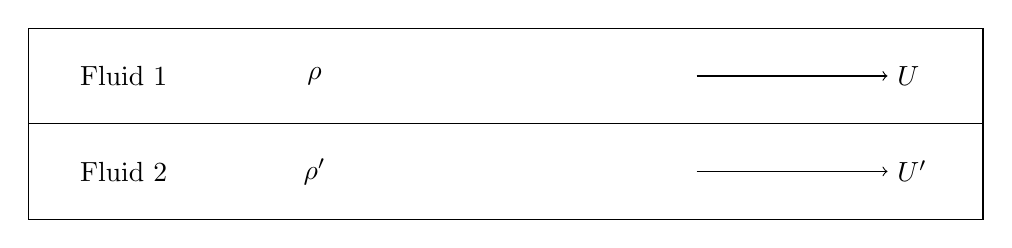
\begin{tikzpicture}[x = \columnwidth/10, y = -\columnwidth/10]
  \draw (0,0) rectangle (10,1);
  \draw (1,0.5) node {Fluid 1};
\draw (3,0.5) node {$\rho$};
  \draw [->] (7,0.5) -- (9,0.5) node [right] {$U$};
  \draw (0,1) rectangle (10,2);
  \draw (1,1.5) node {Fluid 2};
\draw (3,1.5) node {$\rho'$};
  \draw [->] (7,1.5) -- (9,1.5) node [right] {$U'$};
\end{tikzpicture}

From equation (\ref{eq:38}) we have
\begin{equation}
  \label{eq:48}
  \nabla F(t) = \nabla \qty( -\pdv{\phi}{t} + \half \vec{v}^2 + \frac{p}{\rho} + \psi) = 0
\end{equation}
So $F(t)$ is constant throughout space, and $\psi = gz$ is the
gravitational potential. We introduce a perturbation, $\xi(x,z,t)$,
and using equation (\ref{eq:48}) conclude that the pressure on either
side is
\begin{subequations}
  \begin{align}
    p' &= - \rho' \qty( - \pdv{\phi}{t} + \half \vec{v}'^2 + gz ) + \text{constant} \\
p &= - \rho \qty(\pdv{\phi}{t} + \half \vec{v}^2 + gz ) + \text{constant}
  \end{align}
\end{subequations}
At the interface these must be equal, so at $z=\xi$,
\begin{equation}
  \label{eq:49}
   \rho' \qty( - \pdv{\phi}{t} + \half \vec{v}'^2 + g \xi ) = \rho \qty(\pdv{\phi}{t} + \half \vec{v}^2 + g\xi ) + K(t)
\end{equation}
for spatial constant $K$. If we impose a boundary condition that at
all times the perturbation tends to $0$ as $z$ increases then $K$ is
constant in time too.

To find $K$ consider the unperturbed case with $\xi=0$, so
\begin{align*}
  \phi&=0 & \phi' &= 0 \\
v &= U & v' &= U'
\end{align*}
again, as pressures balance at the interface,
\begin{equation}
  \label{eq:50}
  K = \rho \frac{U^2}{2} - \rho' \frac{U'^2}{2}
\end{equation}
so, for a small $\xi$, and given that $\vec{v} = U \vec{e}_x - \nabla \phi$,
\begin{subequations}
  \begin{align}
    v^2 &= (U \vec{e}_x - \nabla \phi)^2 = U^2 - 2 U \pdv{\phi}{x} + \cdots \\
v'^2 &= (U' \vec{e}_x - \nabla \phi)^2 = U'^2 - 2 U' \pdv{\phi'}{x} + \cdots
  \end{align}
\end{subequations}
Hence
\begin{equation}
  \label{eq:51}
  \rho \qty(-\pdv{\phi}{t} - U \pdv{\phi}{x}+ g \xi) = \rho' \qty(- \pdv{\phi'}{t} - U' \pdv{\phi'}{x} + g \xi)
\end{equation}
Introducing small perturbations,
\begin{subequations}
  \begin{align}
    \xi &= A \exp( - i \omega t + i k x) \\
  \phi &= C \exp( - i \omega t + i k x + kz) \\
  \phi' &= C' \exp( - i \omega t + i k x - kz) 
  \end{align}
\end{subequations}
If $\phi$ and $\phi'$ are perturbations on the velocity potential,
then the total velocity potential can be written by redefining the
potential,
\begin{subequations}
  \begin{align}
    -Ux +\phi &\to \phi \\
-U' x + \phi' &\to \phi'
  \end{align}
\end{subequations}
Then the Lagrangian derivative of $\xi$ is
\begin{equation}
  \label{eq:52}
  \dv{\xi}{t} = v_z = - \pdv{\phi}{z}
\end{equation}
So
\begin{subequations}
  Below the surface
  \begin{equation}
    \label{eq:53}
    - \pdv{\phi}{z} = \pdv{\xi}{t}+U \pdv{\xi}{x}
  \end{equation}
and above it
\begin{equation}
  \label{eq:54}
  - \pdv{\phi'}{z} = \pdv{\xi}{t} + U' \pdv{\xi}{x}
\end{equation}
\end{subequations}
Substituting the equations for $\xi$, $\phi$, and $\phi'$ we get
\begin{subequations}
  \begin{align}
    iA (-\omega +kU) &= -k C \\
iA (-\omega +kU') &= k C' \\
\rho(-iC (-\omega +kU) +gA) &= \rho'(-iC'(-\omega+kU')+gA)
  \end{align}
\end{subequations}
These can be solved for $\omega(k)$, and
\begin{equation}
  \label{eq:55}
  \rho (-\omega + kU)^2 + \rho' (-\omega + kU')^2 = kg(\rho-\rho')
\end{equation}
so
\begin{fequation}[Two-fluid Interface Dispersion Relation]
  \label{eq:two-fluid}
  \frac{\omega(k)}{k} = \frac{\rho U + \rho'U'}{\rho+\rho'} \pm \qty( \frac{g}{k} \frac{\rho-\rho'}{\rho+\rho'} - \frac{\rho \rho'(U-U')^2}{(\rho+\rho')^2} )^{\half}
\end{fequation}

There are now a number of ways of producing instabilities. In summary
\begin{description}
\item[Rayleigh-Taylor] Fluids at rest, when $\rho < \rho'$
\item[Kelvin-Helmholtz] When $\rho \rho' (U-U')^2 > \frac{g}{k} (\rho^2 - \rho'^2)$
\item[Jeans Instability] When $\omega^2 = c~S^2 (k^2 - k~J^2)$
\end{description}

\subsection{Rayleigh-Taylor instability}
\label{sec:rayl-tayl-inst}

Let the two fluids be at rest, so $U=U'=0$, but assume that the denser
fluid is above the lighter one, so $\rho<\rho'$. This is intuitively
an unstable equilibrium. The dispersion relation has a solution
\begin{equation}
  \label{eq:57}
  \frac{\omega(k)}{k} = \pm \sqrt{\frac{g}{k} \frac{\rho-\rho'}{\rho+\rho'}}
\end{equation}
for the situation $\rho<\rho'$ we find there is an imaginary part of
$\omega/k$, so
\[ \xi = A \exp(-i \omega t + i k x) = A e^{( \Im(\omega) t) }e^{ -i
\Re(\omega) t + i k x} \] When $\Im(\omega)>0$ the small perturbation
grows exponentially in time, producing an instability.

\subsection{Kelvin-Helmholtz instability}
\label{sec:kelv-inst}

Consider the case where $U \neq U' \neq 0$, but $\rho > \rho'$. The
square-root of equation (\ref{eq:two-fluid}), and so the frequency
$\omega$ is complex, so we get an instability if
\begin{equation}
  \label{eq:58}
  \rho \rho' (U-U')^2 > \frac{g}{k} (\rho^2-\rho'^2)
\end{equation}
Thus
\begin{equation}
  \label{eq:59}
  k > g \frac{\rho^2 - \rho'^2}{\rho \rho' (U - U')^2} 
\end{equation}
is the condition for the instability to occur; as a result it is
possible to avoid the instability at sufficiently long wavelengths.

\subsection{Acoustic waves}
\label{sec:acoustic-waves}

Consider a homogeneous perfect gas with density $\rho_0$ and pressure
$p_0$, then the hydrodynamic equations for a compressible ($\nabla
\vec{v} \neq 0$) without gravity become
\begin{subequations}
  \begin{align}
\label{eq:61}
    \pdv{\rho}{t} + \nabla(\rho \vec{v}) &= 0 \\
\label{eq:62}
\rho \qty( \pdv{t} + (\vec{v} \vdot \nabla) ) \vec{v} &= - \nabla p
  \end{align}
\end{subequations}
Now, we introduce a pressure perturbation, $p = p_0 + \delta p$ and a
density perturbation $\rho = \rho_0 + \delta \rho$. The perturbations
generate a velocity field $\vec{v} = \delta \vec{v}$ assuming there
are no flows in the gas initially, so $\vec{v}_0 = 0$. Substituting
these into the continuity equation
\begin{equation}
  \label{eq:60}
  \pdv{t}(\rho_0 + \delta \rho) + \nabla \qty( (\rho_0 + \delta \rho) \delta \vec{v}) = 0
\end{equation}
Then, as $\rho_0$ is constant,
\[ \pdv{\delta p}{t} + \rho_0 \nabla \vdot \delta \vec{v} = 0 \] with
only the linear components retained. Then, from Euler's equation (\ref{eq:62})
\[ (\rho_0 + \delta \rho) \qty( \pdv{t} + (\delta \vec{v} \vdot \nabla)) \delta \vec{v} = - \nabla (p_0 + \delta p) \]
Which linearises to
\begin{equation}
  \label{eq:64}
  \rho_0 \pdv{\delta \vec{v}}{t} = - \nabla \delta p
\end{equation}
Solving the linear continuity and Euler equations requires a relation
between $\delta p$ and $\delta \rho$, which is the equation of
state. In a perfect gas the motion is adiabatic, so
\begin{equation}
  \label{eq:65}
  \delta p = \eval{\pdv{p}{\rho}}_{p = p_0} \delta \rho
\end{equation}
Using this relation between the density and pressure perturbations the
system of equations becomes
\begin{subequations}
  \begin{align}
    \pdv{\delta \rho}{t} + \rho_0 \nabla \vdot \delta \vec{v} &= 0 \\
\pdv{\delta \vec{v}}{t} &= - \frac{1}{\rho_0} \eval{\pdv{p}{\rho}}_{p=p_0} \nabla \delta \rho
  \end{align}
\end{subequations}
Differentiating the second equation with respect to time, and
substituting from the first equation,
\[ \pdv[2]{\delta \vec{v}}{t} = - \frac{1}{\rho_0} \eval{\pdv{p}{\rho}}_{p=p_0} \nabla \pdv{\delta \rho}{t} = \eval{\pdv{p}{\rho}}_{p=p_0} \Lap \delta \vec{v} \]
Thus we obtain a wave equation for $\delta \vec{v}$, 
\begin{equation}
  \label{eq:66}
  \pdv[2]{\delta \vec{v}}{t} - c~s^2 \Lap \delta \vec{v} = 0
\end{equation}
With $c~s$ the sound speed. The adiabatic gas law,
\[ p = p_0 \qty( \frac{\rho}{\rho_0} )^{\gamma} \] the sound speed can
be expressed in terms of the unperturbed fluid, so
\[ c~s^2 = \eval{\pdv{p}{\rho}}_{p=p_0} = \gamma \frac{p_0}{\rho_0} = \gamma \frac{k~B T}{m} \]
for $k~B$ the Boltzmann constant, since $p = \rho k~B T /m$.

Now, for the dispersion relation, consider a plane-wave perturbation,
$\delta \vec{v} \propto \exp(-i \omega t + i \vec{k} \vdot \vec{r})$; substituting this into the wave equation,
\begin{equation}
  \label{eq:67}
  \omega^2 = c~s^2 k^2
\end{equation}

\subsection{Jeans instability}
\label{sec:jeans-instability}

In the case that a fluid is self-gravitating, we can investigate a
perturbation of the gravitational potential. Let $\psi = \psi_0 +
\delta \psi$ be a perturbed gravitational potential, then
\[ - \nabla p_0 - \rho_0 \nabla \psi_0 = 0 \] with
\[ \Lap \psi_0 = 4 \pi G \rho_0 \] For an infinite gas there are no
nn-trivial uniform solutions, and for $\psi_0$ constant we find
$\rho_0 = 0$. However, if we assume there is an additional force
producing an equilibrium, perturbing and linearising the continuity
equation results in
\[ \pdv{\delta \rho}{t} + \rho_0 \nabla \delta \vec{v} = 0 \]
Linearising the Euler equation, then subtracting the equilibrium
equation, $\nabla p_0 = - \rho_0 \nabla \psi_0$,
\[ \rho_0 \pdv{\delta \vec{v}}{t} = -c~s^2 \nabla \delta \rho - \rho_0 \nabla \delta \psi \]
Similarly, subtracting the equilibrium force from the Poisson equation,
\begin{equation}
  \label{eq:68}
  \Lap \delta \psi = 4 \pi G \delta \rho
\end{equation}
Letting the perturbations vary as $\exp(-i \omega t + i \vec{k} \vdot
\vec{r})$ we have the system of linear equations
\begin{subequations}
  \begin{align}
    - \omega \delta \rho + \rho_0 \vec{k} \delta \vec{v} &= 0 \\
- \rho_0 \omega \delta \vec{v} &= - c~s^2 \vec{k} \delta \rho - \rho_0 \vec{k} \delta \psi \\
- k^2 \delta \psi &= 4 \pi G \delta \rho
  \end{align}
\end{subequations}
Combining these, and eliminating the $\delta$-terms, we find
\begin{equation}
  \label{eq:69}
  \omega^2 = c~s^2 k^2 - 4 \pi G \rho_0 = c~s^2 (k^2 - k~J^2)
\end{equation}
for $k~J^2 = 4 \pi G \rho_0 / c~s^2$. For all $k < k~J$ we find
$\omega$ must be imaginary, producing an instability, the Jeans
instability. Hence a perturbation with a wavelength
\[ \lambda > \lambda~G = \frac{2 \pi}{k~J} = c~s \sqrt{\frac{\pi}{G
    \rho_0}} \] has enough self-gravity to overpower the excess
pressure. The corresponding \emph{Jeans mass} is the mass of a
spherical volume with a diameter of one Jeans wavelength,
\begin{equation}
  \label{eq:70}
  M~J = \frac{4 \pi}{3} \rho_0 \qty( \frac{\lambda~J}{2})^3 = \frac{\pi^{5/2}}{6} \frac{c~s^3}{G^{3/2} \rho_0^{1/2}}
\end{equation}
Given that $c~s^2 = \gamma k~B T/m$,
\begin{equation}
  \label{eq:71}
  \lambda~J = \sqrt{\frac{\gamma \pi k~B T}{m G \rho_0}}
\end{equation}
and
\begin{equation}
  \label{eq:72}
  M~J = \frac{\pi^{5/2}}{6 \rho_0^{1/2}} \qty( \frac{\gamma k~B T}{m G} )^{3/2}
\end{equation}

\section{Shockwaves}
\label{sec:shockwaves}

When the amplitude of a wave is not small the procedure of splitting
the perturbed and unperturbed fluid variables ceases to be
valid. Consider a one-dimensional density wave with $\vec{v} =
(v,0,0)$, so the Euler equation is
\begin{equation}
  \label{eq:56}
  \pdv{v}{t} + v \pdv{v}{x} = - \frac{1}{\rho} \pdv{p}{x}
\end{equation}

We need the other hydrodynamic equations to make any headway, but
simplifying things slightly,
\begin{equation*}
  \pdv{v}{t} + v \pdv{v}{x} = 0
\end{equation*}
and considering its integral curves, $\dv*{x}{t} = v$ in the
$(x,t)$-plane we find the total derivative of $v$ along one of these
curves to be
\[ \dv{t} v(x(t),t) = \pdv{v}{t} + \pdv{v}{x} \dv{x}{t} \]
so along any curve $\dv*{x}{t}=v$ we find $\dv*{v}{t}=0$.

In the simplification of equation (\ref{eq:56}) the solution has the
form \[ v(x,t) = v(x-vt) \] which says that the larger the velocity
$v$ the larger the wave amplitude. As a result of the non-linear
component, $(\vec{v} \vdot \nabla) \vec{v}$ in Euler's equation the
wave-front is steepened, forming a shock-front.

Now consider the pressure term, $\nabla p$,
\[ \pdv{v}{t} + v \pdv{v}{x} = - \frac{1}{\rho} \pdv{p}{x} \]
and the one-dimensional continuity equation,
\[ \pdv{\rho}{t} + \pdv{v \rho}{x} = 0 \] These two equations can be
re-written in a more symmetric form,  with $p = p(\rho)$, and
$c~s^2(\rho) = \pdv*{p}{\rho}$ and $\chi = \log(\rho)$

\begin{subequations}
  \begin{align}
    \pdv{v}{t} + v \pdv{v}{x} &= - c~s^2 \pdv{\chi}{x} \\ 
\pdv{\chi}{t} + v \pdv{\chi}{x} &= - \pdv{v}{x}
  \end{align}
\end{subequations}
Multiplying through the continuity equation by $c~s(\rho)$ we can
combine these
\begin{equation}
  \label{eq:63}
  \pdv{v}{t} + (v+c~s) \pdv{v}{x} = - c~s \qty( \pdv{\chi}{t} + (v + c~s) \pdv{\chi}{x})
\end{equation}
So the disturbance travels at a speed $(v+c~s)$. If the amplitude of
the wave is small $v$ can be neglected, but density fluctuations
propagate with a constant speed $c~s$. When the amplitude is larger
the velocity $v$ becomes important, and the solution becomes
non-linear. The characteristic velocities
\[ \dv{x}{t} = v \pm c~s \]
give the trajectories of the fluid elements along which the quantities 
\[ v \pm \int \frac{c~s}{\rho} \dd{\rho} \] are conserved. These are
Riemann invariants.

\section{Rankine-Hugoniot conditions}
\label{sec:jump-cond-envel}

A shockwave is a thin region of the fluid where dynamic variables
change rapidly. Consider the discontinuity across which various
hydrodynamic variables ``jump''.
% \begin{tikzpicture}[x = \columnwidth/10, y=-\columnwidth/10]
%   \draw (5,0) -- (5,2);
% \draw (4,1) node {$v_1$};
% \draw [->](0,0.5) -- (4.5,0.5); \draw [->] (0, 1.5) -- (4.5, 1.5);
% \draw (6,1) node {$v_1$};
% \end{tikzpicture}
Consider a shock propagating in a medium with density $\rho_1$ and at
a pressure $p_1$ in the shock rest frame. The one-dimensional
hydrodynamic equations are then, in a conservative form,
\begin{subequations}
  \begin{align}
    \pdv{\rho}{t} + \nabla_x (\rho v) &= 0\\
\pdv{\rho v}{t} + \nabla_x(\rho v^2 + p) &= 0\\
\pdv{E}{t} + \nabla_x ([E+p]v)&=0
  \end{align}
\end{subequations}
For \[E = \rho \epsilon + \frac{\rho v^2}{2} \] the total energy per
unit volume, and the shock propagates in the $x$-direction. We assume
the process to be adiabatic, so $p = \rho^{\gamma}$ for $\gamma$ the
adiabatic index, and so
\[ p = (\gamma-1) \rho \epsilon \]
closes the system.

In steady conditions we expect the mass, momentum, and energy fluxes
to be conserved, and at the shock front discontinuity these must also
be conserved. If the shock propagates into a region at density
$\rho_2$ and with pressure $p_2$, then
\begin{align*}
  \rho_1 v_1 &= \rho_2 v_2 \\
\rho_1 v_1^2 + p_1 &= \rho_2 v_2^2 + p_2 \\
\half v_1^2 + \frac{\gamma p_1}{(\gamma-1)\rho_1} &= \half v_2^2 + \frac{\gamma p_2}{(\gamma-1) \rho_2}
\end{align*}
Let us now define the Mach number,
\begin{fequation}[Mach Number]
  \label{eq:73}
  M = \frac{v}{c~{s}} = \frac{v}{\sqrt{\frac{\gamma p}{\rho}}}
\end{fequation}
which is the ratio of the velocity of propagation to the velocity of
pressure wave (sound) propagation, then we can also define the
compression ratio,
\begin{equation}
  \label{eq:74}
  \frac{\rho_2}{\rho_1} = \frac{(\gamma+1)M_1^2}{2+(\gamma-1)M_1^2}
\end{equation}
Clearly, as $M_1 < 1$ this ratio is less than 1, and the shock
disappears, but when $M_1>1$ the ratio grows with $M_1$, and the shock
front forms. $\rho v$ must be constant, so a stronger compression must
move faster, and so the pressure ratio becomes
\begin{equation}
  \label{eq:75}
  \frac{p_1}{p_2} = \frac{(\gamma+1) - (\gamma-1) \rho_2/\rho_1}{(\gamma+1)\rho_2/\rho_1 - (\gamma-1)}
\end{equation}

The equations which relate the variables before and after the shock front are the Rankine-Hugoniot conditions. The density compression has a limiting value for $M \to \infty$,
\begin{equation}
  \label{eq:76}
  \frac{\rho_2}{\rho_1} \to \frac{\gamma+1}{\gamma-1}
\end{equation}
For a monatomic gas $\gamma = \frac{5}{3}$, so the maximum $\rho_2/\rho_1 = 4$. In a diatomic gas $\gamma \approx 1.4$ so $\rho_2/\rho_1 = 6$.

\section{Supernova remnant expansion}
\label{sec:supern-remn-expans}

The expansion of a supernova remnant evolves in three phases,
\begin{enumerate}
\item Free expansion --- ejecta expands without decelerating, so $r \propto t$
\item Adiabatic (Sedov-Taylor) expansion --- energy is conserved
\item Radiative expansion --- energy is disappated into the interstellar medium
\end{enumerate}

\subsection{The Sedov-Taylor regime}
\label{sec:sedov-taylor-regime}

A sudden explosion of gas in a localised region produces a spherical
shockwave which spreads outwards. The Rankine-Hugoniot conditions must
hold across the shock front,so consider the energy $E$, which is
released suddently into a pressureless medium with density $\rho_0$
($p_0 \approx 0)$. $\lambda$ is the scale parameter which describes
the size of the blast wave at a time $t$ after the explosion,
\begin{equation}
  \label{eq:77}
  \lambda = \qty( \frac{E t^2}{\rho_0})^{\frac{1}{5}}
\end{equation}
The radius of the shell just evolve in the same way as $\lambda$, so
\begin{equation}
  \label{eq:78}
  r~s(t) = \zeta_0 \qty( \frac{E t^2}{\rho_0})^{\frac{1}{5}}
\end{equation}
The velocity evolves as
\begin{equation}
  \label{eq:79}
  v~s(t) = \dv{r~s(t)}{t} = \frac{2}{5} \frac{r~s(t)}{t} = \frac{2}{5} \zeta_0 \qty(\frac{E}{\rho_0 t^3})^{1/5}
\end{equation}
Thus the size of the spherical blast increases as $t^{2/5}$ but the
velocity falls off as $t^{-3/5}$. This is the Taylor-Sedov expansion
for an adiabatic blast wave. A typical supernove ejects around $1
M_{\odot}$ of material at a velocity of
$10^4\,\kilo\meter\,\second^{-1}$, so has an energy $E\sim
10^{44}\,\joule$ assuming the material has a density of
$2\e{-21}\,\kilogram\,\meter^{-3}$. Thus, assuming $\zeta_0=1$,
\begin{subequations}
\begin{equation}
  \label{eq:80}
  r~s (t) \approx 0.3 \qty( \frac{t}{1\,\text{year}} )^{2/5}\,\text{pc}
\end{equation}
\begin{equation}
  \label{eq:81}
  v~s (t) \approx 10^5 \qty(\frac{t}{1\,\text{year}})^{-3/5}\,\kilo\meter\,\second^{-1}
\end{equation}
\end{subequations}
These relations become invalid after around $10^5$ years due to the
cooling of the ejecta, but are a very good approximation for the first
hundred years of expansion.

\section{Particle acceleration by supernovae}
\label{sec:part-accel-supern}

The first cosmic rays were observed in 1902 in a railway tunnel
outside Peebles, Scotland by CTR Wilson, but the first correct
determination that these particles were of cosmic origin was due to V
Hess in 1912, from a $5\,\kilo\meter$ balloon experiment. Since then
indirect measurements of the particles from supernova remnants have
been made through their synchrotron emission in the x-ray regime.

\subsection{Fermi acceleration}
\label{sec:fermi-acceleration}

Consider a relativistic particle reflecting from a moving mirror. If $\vec{v}~s$
is the velocity of the shock structure (which acts as the magnetic mirror) then the change in energy for the particle when reflected, $\Delta E$, is 
\[ \Delta E = - 2E \frac{\vec{v}~s \vdot \vec{v}_{\parallel}}{c^2} \]
For $c$ the speed of light. Assuming an isotropic distribution of
energetic ultra-relativistic particles, we find the energy given to a
particle by the shock is
\[ \frac{\ev{\Delta E}}{E} = \frac{4}{3} \frac{v~s}{c} \] Let us now
assume that there are a large number of shock fronts moving randomly
in all directions. The probability of a head-on collision is
proportional to $v~s + v$, while the probability of overtaking a
collision is proportional to $v- v~s$. Thus
\begin{equation}
  \label{eq:82}
  \ev{ \Delta E} = \frac{v+v~s}{2 v} \Delta E - \frac{v-v~s}{2 v} \Delta E \approx 2 \frac{v~s^2}{c^2} E
\end{equation} 
The average rate of energy gain is
\begin{equation}
  \label{eq:83}
  \dv{E}{t} = \frac{\ev{\Delta E}}{\tau} = 2 \frac{v~s^2}{\tau c^2} E 
\end{equation}
Where $\tau$ is the time between collisions. The energy thus increases
linearly with time,
\begin{equation}
  \label{eq:84}
  E(t) = E_0 \exp( \frac{2 v~s^2}{\tau c^2})
\end{equation}
Let $E = bE_0$ be the average energy of a particle after one
collision, and $P$ the probability that the particle remains within
the acceleration region after one collision. After $k$ collisions
there will be $N = N_0 P^k$ particles with energies above $E =
b^kE_0$, so
\begin{equation}
  \label{eq:85}
  \frac{N}{N_0} = \qty( \frac{E}{E_0} )^{\log(P) / \log(b)}
\end{equation}
so 
\begin{equation}
  \label{eq:86}
  N(E) \propto E^{-1 + \log(P)/\log(b)}
\end{equation}
so the energy distribution of particles has a power-law distribution.

\section{The canonical model of shock acceleration}
\label{sec:canon-model-shock}

Consider the idealised problem of a particle accelerated by a shock
wave with one-dimensional geometry propagating in a medium containing
small-scale magnetic-field inhomogeneities which scatter fast-moving
particles.

Provided that the scattering of fast particles is strong enough to
ensure the isotropy assumption the kinetic equation for relativistic
particles in the stationary diffusion-advection equation is
\begin{equation}
  \label{eq:87}
  \pdv{x} v N = \pdv{x} D \pdv{N}{x} + \frac{1}{3} \pdv{v}{x} \pdv{E} E N
\end{equation}
for $N(E,x)$ the energy distribution of the particles, $v(x)$ the
velocity of the stream, and $D$ the spatial diffusion of the energetic
particles. Thus $E \approx pc$ for $p$ the particle
momentum. Integrating over $x$, with the boundary conditions
\begin{align*}
  N(E)=N_1(E) && v=v_1 && \text{at } x \to - \infty\\
N(E) = N_2(E) && v=v_2 && \text{at } x \to + \infty
\end{align*}
From the integration
\[ v_2 N_2(E) - v_1 N_1(E) + 0 - 0 = \frac{1}{3} (v_2 - v_1) \pdv{E} E N_2(E,x) \]
Then the down-stream particle distribution, $E_2(E)$ is given by the ODE
\begin{equation}
  \label{eq:88}
  N_2(E) = \frac{3}{R-1} E^{-\delta} \int^E_{E_0} N_1(E') E'^{\delta-1} \dd{E'} + C E^{- \delta}
\end{equation}
for $C$ some constant, and $\delta = (R+2)/(R-1)$ the spectral index
of the distribution.  When \[N_1(E) = N_0 \delta(E-E_0) \] from an
injection of particles at energy $E_0$,
\[ N_2(E) \propto E^{-\delta} \] for $E>E_0$. 

In strong shockwaves $R = 3$ to $R=4$, so $\delta = 2$ to
$\delta=2.5$. In cosmic rays the spectrum of ions is an un-broken
power law between $10^9\,\electronvolt$ and $10^6\,\electronvolt$, and
with $\delta \approx 2.6$. As a result supernova shockwaves are one of
the leading candidates to explain the production of these particles.

%%% Variables: 
%%% mode: latex
%%% TeX-master: "../project"
%%% End: 


\chapter{Supernovae}
\label{cha:supernovae}
A supernova is the explosion which occurs at the end of the lifespan
of a star, which produces a sufficient quantity of energy to outshine
its host galaxy for a brief time. There are other mechanisms for the
ignition of a supernova, however.

\begin{table*}
\centering
\begin{tabular}{l ll l}
\toprule
Main Class                & Sub-class & Features                                                           & Mechanism                      \\ 
\midrule
  \multirow{3}{*}{Type I} & Ia        & Si II line.                                                        & Thermal runaway                \\
                          & Ib        & Weak or no Si, He I line.                                          & \multirow{2}{*}{Core collapse} \\
                          & Ic        & Weak or no Si, no He.                                              &                                \\
\midrule
\multirow{4}{*}{Type 2}   & II-P      & Type II spectrum, No narrow lines, light curve plateaus.           & \multirow{4}{*}{Core collapse} \\
                          & II-L      & Type II spectrum, no narrow lines, light curve decreases linearly. &                                \\
                          & II-n      & Type II spectrum, some narrow lines.                               &                                \\
                          & II-b      & Spectrum changes to become Type Ib-like spectrum.                  &                                \\
\bottomrule
\end{tabular}
\caption{A summary of the classifications of supernova.}
\label{tab:supernova-category}
\end{table*}

There are a number of different classifications of supernovae (these
are summarised in table \ref{tab:supernova-category}), with the
subdivisions made based on spectral properties of the explosion.

\section{Type I }
\label{sec:type-i-}

If a supernova does not show Balmer lines from hydrogen it is
categorised as a type I supernova, and then sub-divided based on the
silicon and helium lines.

\subsection{Type-Ia}
\label{sec:type-ia}

Type Ia supernovae show helium and silicon ion absorption lines, and
are believed to arise as a result of mass accretion onto a white dwarf
in a binary system. This causes the white dwarf to exceed the
Chandrasekhar mass limit, and collapse to a neutron star. The
consensus view, however, is that for a period of just 1000 years, when
the white dwarf has around 99\% of the limit mass, convection occurs,
allowing deflagration through carbon and later oxygen
fusion. Degeneracy pressure is independent of temperature, and so the
fusion process is prone to runaway, and Rayleigh-Taylor instability
causes the burning surface to accelerate dramatically.

A second mechanism arises in systems with two degenerate white dwarfs,
which eventually coalesce, forming a super-Chandrasekhar star, which
then collapses to form a neutron star.

\subsection{Types-Ib and -Ic}
\label{sec:types-ib-ic}

Types-Ib and -Ic are the result of the collapse of massive stars which
have undergone a red-giant phase, and have lost most of their outer
layer of hydrogen and helium gas. They have a low occurrence rate
thanks to the scarcity of massive stars in the Galaxy.

\section{Type II}
\label{sec:type-ii}

Type II supernovae are the ``normal'' supernovae, for progenitors with
8 to 40 times the mass of the Sun, and represent the result of core
collapse, due to the inability of the progenitor to balance the
gravitational pressure of the gas by thermodynamic pressure from the
nuclear reactions in the core.

Type IIP supernovae, which show a plateau in their lightcurves, are
the result of the collapse of a star with a hydrogen envelope with
$M\ge 2M_{\odot}$, whereas IIL supernovae have less massive envelopes,
which cannot sustain the plateau.

\section{Late phase evolution}
\label{sec:late-phase-evolution}

The pressure generated in the core of a star must balance the weight
of the material composing a star to prevent collapse. In the Newtonian
regime this is described by the relation
\begin{equation}
  \label{eq:126}
  \pdv{P}{r} = - \frac{G M(r) \rho(r)}{r^2}
\end{equation}
for $P$ the pressure at a radius $r$ from the star's centre, and
$\rho(r)$ the density. In polytrophic models of stars
\[ P \propto \rho^{(n+1)/n} \]
thus
\begin{equation}
  \label{eq:127}
  \frac{P~c^3}{\rho~c^4} = 4 \pi G^3 \qty( \frac{M}{\phi} )^2
\end{equation}
for the central density and pressure, and $\phi$ the constant of
proportionality,
\begin{equation}
  \label{eq:128}
  \phi(n) =
  \begin{cases}
    4.9 & \text{ for } n=0 \\
10.7 & \text{ for } n= 1.5 \\
16.15 & \text{ for } n = 3 
  \end{cases}
\end{equation}

As a star runs out of fuel for a given fusion process it will
contract, and its temperature will increase, allowing a higher-order
fusion process to be undertaken, pausing the contraction process,
however, after helium burning the temperature in the star is
sufficient to maintain a large population of thermalised electrons and
positrons, which can annihilate to form a neutrino-antineutrino
pair. The loss of this mass accelerates the contraction process, and
so, while helium burning may last many years, silicon burning lasts
only a few weeks.

\section{Mass loss}
\label{sec:mass-loss}

The final evolution of a star is highly dependent upon the amount of
mass which is lost in the late stages of its evolution, and this is
dependent upon the star's metallicity. The mass loss is wind-driven in
large stars, and since this has a strength proportional to the square
root of the abundance of metals it becomes a dominant effect in very
metallic stars. If the star loses its entire Hydrogen envelope its
rate of mass loss can increase significantly, producing a turning
point in figure \ref{fig:remnants}, as much smaller helium cores
remain at the time of the star's collapse.


\begin{figure*}
  \centering
    \begin{tikzpicture}
    \begin{semilogxaxis}[xmin=8, xmax=300, 
                         ymin= 0, ymax=1, 
                         width=\textwidth, height=8cm,
                         xlabel=Initial mass ($M_\odot$), ylabel=log(metallicity)]
      \draw (axis cs: 5,0.5) node {1};

      \fill [muted-blue!40]
      (axis cs: 9,0) -- (axis cs: 9,1) -- (axis cs: 10, 1) -- (axis cs: 10,0) -- cycle;


      \fill [muted-blue!90]
      (axis cs: 39, 0) -- (axis cs: 39, 0.8) -- (axis cs: 300, 0.8) -- (axis cs: 300, 0) -- cycle;

      \fill [muted-blue!70]
      (axis cs: 40,0) -- (axis cs: 40, 0.6) -- (axis cs: 100,0.5) -- (axis cs: 200,0.6) -- (axis cs: 300, 0.7) -- (axis cs: 300, 1) -- (axis cs: 10, 1) -- (axis cs: 10, 0) -- cycle;


      \fill [muted-blue!20]
      (axis cs: 25,0) -- (axis cs: 25, 0.5) -- (axis cs:30,0.8) -- (axis cs: 34, 0.9)
   -- (axis cs: 80,0.8) -- (axis cs: 260,0.9) -- (axis cs: 300, 0.99) 
   -- (axis cs: 300, 1) -- (axis cs: 10, 1 ) --(axis cs:10,0);

      \fill [white] 
      (axis cs: 140,0) -- (axis cs: 260,0) -- (axis cs: 260, 0.2) -- (axis cs: 300, 0.2) -- (axis cs: 300, 0.25) -- (axis cs: 200, 0.25) -- (axis cs: 140, 0.2) -- cycle;

      \draw [ultra thick, black] (axis cs: 32, 1) -- (axis cs: 34, 0.9) -- (axis cs: 40,0.6) -- (axis cs: 120, 0.3) -- (axis cs: 100, 0.2) -- (axis cs:100, 0);
   

      \node at (axis cs: 8.5, 0.5) {\circled{1}};
      \node at (axis cs: 9.5, 0.75) {\circled{2}};
      \node at (axis cs: 15, 0.5) {\circled{3}};
      \node at (axis cs: 30, 0.5) {\circled{4}};
      \node at (axis cs: 60, 0.3) {\circled{5}};
      \node at (axis cs: 200, 0.1) {\circled{6}};
      \node at (axis cs: 280, 0.1) {\circled{7}};

      \node at (axis cs: 39, 0.8) [rotate=-65] {No H envelope.};
      \node at (axis cs: 33, 0.8) [rotate=-65] {\phantom{No }H envelope.};

    \end{semilogxaxis}
  \end{tikzpicture}
%%% Local Variables: 
%%% mode: latex
%%% TeX-master: "../project"
%%% End: 

  \caption{The remnants left by a variety of masses and metallicities.}
  \label{fig:remnants}
\end{figure*}

\section{Low-mass stars}
\label{sec:low-mass-stars}

Low mass stars, with progenitor masses lower than 9 solar masses will
shed the majority of their outer material in their red giant phase,
leaving a Carbon-Oxygen core with a mass of 0.6 to 1.1 solar masses,
which forms a white dwarf; a degenerate remnant supported by electron
degeneracy pressure. This situation is illustrated in figure
\ref{fig:remnants}: the production of a white dwarf by a star with
mass under $<9 M_\odot$ is represented by region \circled{1}. The loss
of mass in the late stages of the star's evolution are important, and
a star with a mass under 11 solar masses can still, if the element
abundances in the core are correct, form an oxygen-neon white dwarf,
thanks to the development of a convective super-wind, and this is
illustrated in region \circled{2}.

\section{High-mass stars}
\label{sec:high-mass-stars}

In high mass stars the electrons in the core do not become degenerate
until the final stages of the burn, and the luminosity of the star,
which will be close to the Eddington limit, remains almost
constant. Stars with a mass up to 100 solar masses will attempt to
fuse iron. This process is endothermic, and so fails to provide the
required pressure to counterbalance the star's gravitational collapse.
The precise remnant left behind depends on a combination of the mass
of the progenitor and its metallicity \cite{2003ApJ...591..288H}.  For
a zero-metallicity star, up to around 40 solar masses the remnant will
be a neutron star (figure \ref{fig:remnants}, section
\circled{3}). Above this, but below 100 solar masses a black hole will
form as material falls back into the core (section \circled{4}). Above
100 solar masses the collapse leads straight to a black hole, with no
supernova (section \circled{5}). Above 140 solar masses the star will
suffer pair-pair pulsational instability, and no remnant will be
produced (section \circled{6}). For extremely massive (greater than
260 solar masses, section \circled{7}) photodisintegration becomes the
dominant cause of the collapse, and the star becomes a black hole
directly, as in section \circled{5}.

\begin{figure*}[t]
  \centering
  \begin{tikzpicture}
    \begin{axis}[xlabel=$\log(T)$, ylabel=$\log(\rho)$,
                       width=0.95\textwidth, height=8cm,
                       xmin=6, xmax=10,
                       enlarge x limits=false,
                       no markers,
                       domain=5:10,
                       ymin=0, ymax=10
                       ]
      \addplot [fill, black!40, thick]{3*x-13.62-8.5} \closedcycle;
      \addplot [fill, black!30, thick]{3*x-13.62-8.5} -- (axis cs:10,10) -- (axis cs:0,10) -- (axis cs: 0,0)-- (current plot begin);
      \addplot+[fill,thick, black!10, domain=9:10] {3*x-20.5} -- (axis cs: 10,10) -- (axis cs: 0,10) -- (axis cs: 0,6.5) -- (current plot begin);
      \addplot[fill, black!20, domain=5:9]{1.5*x-7} -- (axis cs: 6,6.5) -- (current plot begin);

      \addplot [ultra thick, white, domain=0:7.2] {ln(5.7)*(exp(x)/10^6)^(-1/3) -14}
      -- (axis cs: 7.3,0) node [midway, right, white] {CNO};
      \node at (axis cs: 6.3,6) [right, white] {pp};
      \addplot [ultra thick, white] {ln(150)*(exp(x)/10^6)^(-1/3) -30};
      \node at (axis cs: 7.9,6) [right, white] {$3 \alpha$};
      \addplot [ultra thick, white] {ln(100)*(exp(x)/10^6)^(-1/2) -40};
      \node at (axis cs: 9.1, 8) [right, white]{O+O};

      \fill [black] (axis cs: 9.7,0) -- (axis cs: 9.9,0) -- (axis cs: 9.9,10) -- (axis cs:9.7,10)--cycle;
      \node at (axis cs: 9.8, 6) [rotate=-90, white] {Photodisintegration};
      \fill [black] (axis cs:8.5,0) -- (axis cs: 9.5,0) -- (axis cs: 9.5,7) -- (axis cs: 8.8, 4) -- cycle;
      \node at (axis cs: 8.8, 2.5) [white, right] {Pair instability};

      \draw [accent-red, ultra thick] (axis cs:6,0) -- (axis cs:7,3) -- (axis cs: 6,3) node [midway, above, accent-red] {$0.1\,M_\odot$};
      
      \draw [accent-red, ultra thick] (axis cs: 6.5,0) -- (axis cs:8,5) -- (axis cs:6,5) node [midway, below, accent-red] {$1\,M_\odot$};
      \draw [accent-red, ultra thick] (axis cs:7.2,0) -- (axis cs: 9.7, 7.8) node [midway, above, accent-red, rotate=22] {$10\,M_\odot$};
      \draw [accent-red, ultra thick] (axis cs: 8, 0) -- (axis cs: 8.65,2) node [midway, above, accent-red, rotate=22] {$100\,M_\odot$};

      \node at (axis cs: 6.8, 9) {UR Degenrate};
      \node at (axis cs: 6.8, 6) {NR Degenerate};
      \node at (axis cs: 6.8, 1) {Ideal gas};
      \node at (axis cs: 8.0, 1) {Radiation};

    \end{axis}
  \end{tikzpicture}
%%% Local Variables: 
%%% mode: latex
%%% TeX-master: "../project"
%%% End: 

  \caption{The $\log(T)-\log(\rho)$ diagram.}
  \label{fig:logTlogr}
\end{figure*}

\section{Collapse}
\label{sec:collapse}

If the mass of the iron core of the star exceeds the Chandrasekhar
mass limit it will no longer be possible for a star to produce energy,
but loses due to neutrinos still occur. As this happens electrons are
captured by the heavy nuclei, which in turn reduces the (electron
degeneracy) pressure, accelerating the in-fall. The temperature then
rises rapidly, allowing the photodisintegration of the iron nuclei.
\begin{equation}
  \label{eq:129}
  \gamma(100\,\mega\electronvolt) + ^{56}\ce{Fe} \to 13\, ^4\ce{He} + 4 \ce{n}
\end{equation}
This reaction absorbs around $2 \mega\electronvolt$ of energy per
nucleon. At this point the core collapses in near free-fall at around
$0.25 c$. As the process continues the temperature rises to the point
where helium disintegrates intro protons and neutrons, and free
protons capture free electrons to form neutrons. The collapse is
finally halted by the neutron degeneracy pressure when the density
reaches $10^{18}\,\kilogram/\meter^3$. This remnant is a neutron star.

The formation of the neutron star produces a shockwave as the outer
layers of the core continue to collapse, but this eventually stalls as
a result of photodisintegration and neutrino losses. After a few
milliseconds the gas stops expanding back outward, and the
proto-neutron star starts accreting matter at a rate of several solar
masses per minute. If this accretion is able to continue unabated no
supernova occurs, and within around a second the neutron star further
collapses into a black hole. If this does not occur within a few
seconds, however, neutrino losses force the remnant to become a
neutron star.

\subsection{Neutrino production}
\label{sec:neutrino-production}

During the collapse around 10 percent
($7\,\mega\electronvolt/\text{nucleon}$) of the total energy of the
explosion is lost to nuclear processes, while only 1\% of the
$3\e{46}\,\joule$ of gravitational energy is radiated as photons, and
a few percent as kinetic ejecta. The vast majority of the energy is
used to produce neutrinos. The burst of neutrinos from SN\,1987A was
observed by SuperKamiokande, with the burst lasting 13 seconds.

\section{Pair-instability supernovae}
\label{sec:pair-inst-supern}

Stars with a mass greater than 100 solar masses are still produced in
the galaxy, but these will normally have nuclear and
photometrically-powered pulsations which drive their mass loss. These
are, however, suppressed in extreme Population III stars, and maintain
most of their mass through to the end of their helium burning cycle,
resulting in a massive helium core. If the core has a mass greater
than 42 solar masses the star will experience pair-instability; the
result of high-energy gamma rays in the core after carbon burning has
completed, and this causes a pressure drop. For progenitor masses
between 100 and 130 solar masses this results in sequence of
disruptive pulsations which shed mass from the star until it is below
the instability limit, but for masses in excess of this the first
pulse will have enough energy to violently disrupt the star, producing
an explosion. These supernovae are credited with the production of a
nearly solar distribution of heavy elements up to zinc.

\section{Implosion to explosion}
\label{sec:implosion-explosion}

In order to turn the implosive nature of a supernova into the
explosive process which is observed energy is transferred from the
neutrino flux to the outer layers of the star, rather than the
shockwave produced by the formation of the neutron star. The expanding
material from the supernova will then form a shockfront as it travels
through the interstellar medium, however.

The explosion is the main source of the supernova's light curve. An
early peak is produced as the shock breaks through the surface of the
gas, producing strong UV radiation; the lightcurve will then plateau
as the hydrogen-rich envelope expands and cools and recombines. After
this the tail of the lightcurve is driven by the radioactive decay of
$\ce{^{56}Ni}$.

%%% Local Variables: 
%%% mode: latex
%%% TeX-master: "../project"
%%% End: 



\part{Pulsars}
\label{part:pulsars}

\chapter{Discovery \& Overview of Pulsars}
\label{cha:discovery--overview}
Pulsars are highly magnetised neutron stars which have a hot emitting
region on their surface which produces a beam of electromagnetic
radiation. As the neutron star rotates its beam sweeps out across
space, and we see it as a brief, frequent flash, much like a
lighthouse beam.

Pulsars were discovered, accidentally, in 1967 by Jocelyn Bell under
the supervision of Anthony Hewish, while investigating fluctuations in
the flux densities of extragalactic radio galaxies and quasars. This
interplanetary scintillation is caused by the passage of radio waves
through the solar wind, and depend on the angular size of the source,
and promised to give a measure of the cosmological distribution of
radio galaxies, constraining models of galaxy formation.

\section{Early deductions}
\label{sec:early-deductions}

The pulses from the first pulsars to be detected showed no parallax
effects, but did show timing variations due to the Earth's orbit,
hence were far outside the solar system. They sweep through the radio
band, implying that they have been dispersed by the ISM. The amount of
dispersion implies that they are local galactic objects. Their signals
are bright ($\sim 20\,\text{Jy}$), and these vary in strength. The
pulses have a length shorter than $0.016\,\second$, implying a
diameter around $5\,000\,\kilo\meter$.

\section{Derived properties}
\label{sec:derived-properties}

\subsection{Brightness temperature}
\label{sec:brightn-temp}

The brightness temperature of an object is the temperature which
observing the object would produce in an antenna, and is defined
\begin{equation}
  \label{eq:89}
  T~b = \frac{B c^2}{2 \nu^2 k~B}
\end{equation}
for $B$ the brightness, $c$ the speed of light, $\nu$ the frequency of
the radiation, and $k~B$ the Boltzmann constant.

\begin{example}[Brightness temperature of CP1919]
  We assume a distance of $1\,\kilo\text{pc}$ and a diameter of
  $10\,\kilo\meter$, then the solid angle of the source is
\[ \Omega~s \approx \pi \qty( \frac{5\,\kilo\meter}{3\e{16}\,\kilo\meter} ) = 8\e{-32}\,\steradian \]
and the brightness is
\[ B = \frac{S}{\Omega~S} = \frac{20\e{-26}\,\watt\,\meter^{-2}\,\hertz^{-1}}{8\e{-32}\,\steradian} \]
Then
\[ T~b = 10^{30}\,\kelvin \]
\end{example}
Note, the limit on brightness temperature from synchrotron radiation is around $10^{12}\,\kelvin$.

\subsection{Density}
\label{sec:density}

The density of a pulsar can be inferred from the centrifugal force
which its rotation period implies.  Consider the fastest known pulsar,
PSR\,J1748--2446ad, which is in the globular cluster Terzan 5.

\begin{example}[The density of PSR\,J1748--2446ad]
  This pulsar rotates at a rate $\nu = 716\,\hertz$. Using the mass,
  $M$, the radius, $R$, and the rotation rate $\omega = 2 \pi / P$,
  centrifugal breakup occurs if
\[ \omega^2 R > \frac{GM}{R^2} \]
and so, if 
\[ P^2 < \frac{4 \pi R^3}{3} \frac{3 \pi}{GM} \] then the mean
density, $\rho$, is constrained to be \[\rho > \frac{3 \pi}{GP^2} =
7\e{16}\,\kilo\gram\,\meter^{-3} \]
\end{example}

\subsection{Size}
\label{sec:size}

Assuming that the mass of a neutron star is $1.4\,M_{\odot}$, from
this density, the radius must be less than $21\,\kilo\meter$.

\subsection{Magnetic field}
\label{sec:magnetic-field}

Neutron stars have strong magnetic fields; simple arguments based
around the conservation of magnetic flux during the collapse of the
progenitor star suggests $B \sim 10^8\,\tesla$, but more sophisticated
arguments imply $10^9$ to $10^{11}\,\telsa$. Taking the pulsar to be a
rapidly rotating bar magnet, we have radiation emission as if from a
dipole, with luminosity
\begin{equation}
  \label{eq:90}
  L = \frac{\mu_0 \abs{\ddot{m}}^2 \sin[2](\theta)}{6 \pi c^3} = \frac{2 \pi R^6 B~P^2 \omega^4 \sin[2](\theta)}{3 c^3 \mu_0}
\end{equation}
where $B~P$ is the magnetic flux density of the pulsar at the pole,
and $R$ is its radius. These waves are the primary source of radiation
loss, but do not produce the radiation seen in radio. They are below
the local plasma frequency, so are not transmitted away from the
nebula around the pulsar.

\subsection{Radiation braking}
\label{sec:radiation-braking}

The only source of energy for the pulsar is the rotational kinetic
energy of the rotation about the pulsar's axis, about which the moment
of inertia, $I_{zz}$ produces energy
\begin{equation}
  \label{eq:91}
  E = \half I_{zz} \omega^2
\end{equation}
and so
\begin{equation}
  \label{eq:92}
  L = - \dot{E} = - I_{zz} \omega \dot{\omega}
\end{equation}
Thus, radiation brakes the pulsar, so
\begin{equation}
  \label{eq:93}
  \dot{\omega} = - \frac{2 \pi R^6 B~P^2 \sin[2](\theta)}{3 c^3 \mu_0 I_{zz}} \omega^3
\end{equation}
Such a pulsar has a braking index of $n=3$, where the braking index is
defined from the relation
\begin{equation}
  \label{eq:94}
  \dot{\omega} \propto -\omega^n
\end{equation}
The minimum magnetic field can be determined from this and knowledge
of the spin-down rate, 
\[ B~{min} = 3.2\e{15} \qty( P \dot{P} )^{\half}\,\tesla \]

\begin{figure*}
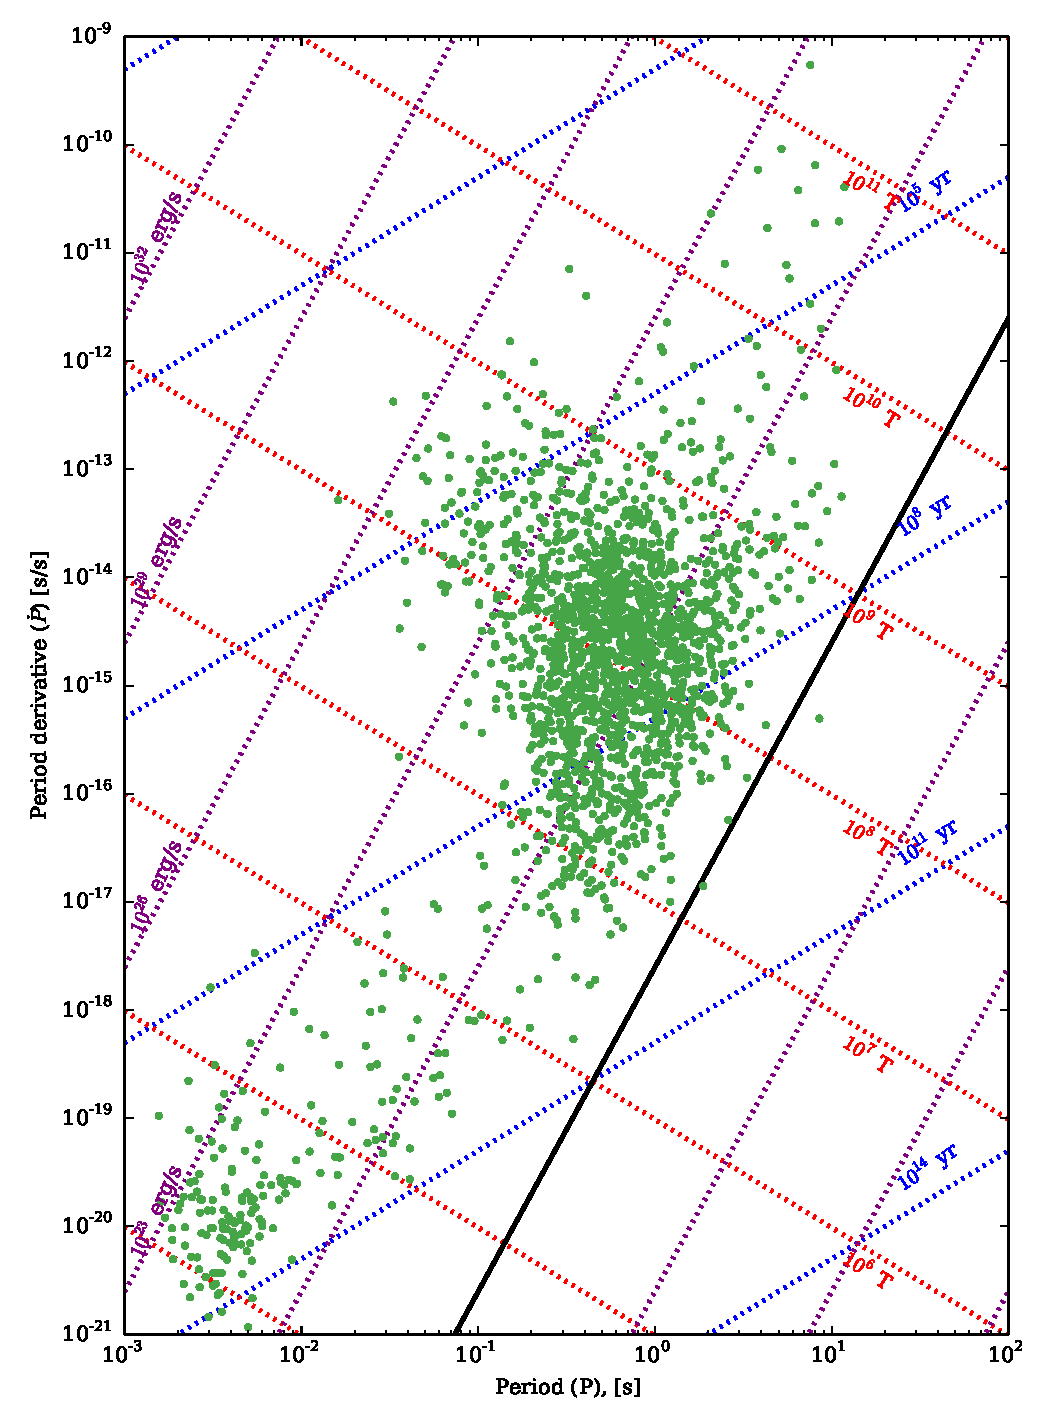
\includegraphics{figures/ppdot.pdf}
\caption{The $P$-$\dot{P}$ diagram of all of the known pulsars, with characteristic ages marked in green.}
\label{fig:ppdot}
\end{figure*}

\subsection{Characteristic age}
\label{sec:characteristic-age}

The characteristic age of a pulsar is an approximation of the age of a
pulsar assuming that it had an initial period smaller than the current
one, has no magnetic field decay, and a braking index of $n=3$. From
this we define the characteristic age, $\tau$, as
\begin{equation}
  \label{eq:95}
  \tau = \frac{P}{2 \dot{P}}
\end{equation}
Allowing for an explicit $n$,
\begin{equation}
  \label{eq:96}
  \tau = \frac{P}{(n-1) \dot{P}} - \frac{P_0}{(n-1) \dot{P}_0}
\end{equation}
for $P_0$ the initial spin period, and $\dot{P}_0$ the initial spin
period derivative.

\subsection{Timing stability}
\label{sec:timing-stability}

The stability of some pulsars' rotation periods rivals that of atomic
clocks over long time periods ($\sim 1\,\text{yr}$), once relative
motion and a constant spin-down rate. At some level all pulsars show
\emph{timing noise}; these may be due to gravitational effects along
the propagation of the wave through space.

\subsection{Astrometric position}
\label{sec:astrometric-position}

Pulsar signals must be Doppler corrected for the relative motion of
the pulsar and the Earth; this correction is sensitive to the position
of the pulsar in the sky. The angular resolution of observations of a
pulsar are equivalent to those of an aperture of radius
$1\,\text{AU}$. Then for a $100\,\hertz$ pulsar,
\[\theta \approx \frac{\lambda}{D} = \frac{c/\nu}{2\,\text{AU}} \approx 2\,\text{as}\]
We can, however measure over many cycles, and so
\[ \theta = \frac{d}{D} = \frac{c \Delta \tau}{2\,\text{AU}} \approx
206 \Delta \tau\,\text{as} \] with the best timing resolutions $\Delta
\tau \approx 50\,\nano\second$, and hence astrometric precisions of
$\theta \approx 10\,\micro\text{as}$.

\subsection{Gravitational physics}
\label{sec:grav-phys}

Binary neutron star systems have two orbiting masses which form a
rotating mass quadrupole, and generate gravitational waves with a
luminosity of
\begin{equation}
  \label{eq:97}
  L~G = \frac{32}{5} \frac{G^4}{c^5} \frac{m_1^2 m_2^2 (m_1+m_2)}{a^5}
\end{equation}
at twice the orbital frequency.

By monitoring the travel times of pulses it is possible to infer the
presence of a gravitational wave. Say a pulse is sent at $(x_1,t_1)$,
and the strain along the line of sight is $h$, then the fractional
change in the arrival rate can be reduced to the difference in the
strain at the start and the end of the transmission,
\begin{equation}
  \label{eq:98}
  \frac{\var{\nu}}{\nu} = h(x_1,t_1) - h(x_2, t_2) 
\end{equation}
This is the only know way to detect very low frequency gravitational
waves, producing a timing residual of
\begin{equation}
  \label{eq:99}
  R(t) = - \int_0^t \frac{\var{\nu}}{\nu} \dd{t}
\end{equation}

\subsection{Equation of state}
\label{sec:equation-state}

Variations in the rotation of pulsars allow the equation of state to
be inferred. The density profile determines the moment of inertia,
\[ I_{zz} = kMR^2 \] for $k=2/5$ for a uniform ball. Glitches indicate
that there is a superfluid internal structure which couples to the
crust, creating steep rotation-rate gradients , deforming the crust.

\subsection{Extreme plasmas}
\label{sec:extreme-plasmas}

Pulsars are a complex problem in relativistic plasma physics, as
neither the radiation mechanism nor the structure of the magnetosphere
is well understood. The plasma of the magnetosphere forms a pulsar
wind nebula, and these are visible in x-ray wavelengths for the crab
and vela pulsars. The double pulsar system, PSR\,J0737-3039, provides
the most sensitive measurements of these nebula, as the pulsar beams
from the two components pass through the other's wind nebula
frequently.

\subsection{Extrasolar planets}
\label{sec:extrasolar-planets}

Periodicities in the timing residuals of PSR\,B1257+12 are consistent
with the gravitational effects of four planets.


%%% Local Variables: 
%%% mode: latex
%%% TeX-master: "../project"
%%% End: 


\chapter{Dispersion and Scintillation}
\label{cha:disp-scint}
The Galaxy is filled with a tenuous plasma, the interstellar medium,
which affects photons which travel through it. In normal observations
this effect isn't visible, since the majority of sources emit light
continuously, but for pulsars it is an important effect, and one which
must be corrected.

\section{Propagation of light in a plasma}
\label{sec:prop-light-plasma}

Consider a wave of angular frequency $\omega$, with the electric
field, with amplitude $E$, described by
\begin{equation}
  \label{eq:100}
  E = E_0 \exp(i \omega t)
\end{equation}
which propagates in a plasma of electron number density
$n~e$. Assuming that the protons are quasi-stationary, the electrons
rotate about them as
\[ x = x_0 \exp(i \omega t) \]
with an equation of motion
\begin{equation}
  \label{eq:101}
  E e = m~e \ddot{x} = -m~e \omega^2 x 
\end{equation}
Charge separation appears as a bulk polarisation, defining the
relative permittivity, $\epsilon~r$, of the plasma,
\begin{equation}
  \label{eq:102}
  P = n~e p = (\epsilon~r -1) \epsilon_0 E
\end{equation} 
for $p = xe$ the dipole moment of a proton-electron pair. Then, using
the equation of motion,
\begin{equation}
  \label{eq:103}
  \epsilon~r = 1 - \frac{n~e e^2}{\epsilon_0 m~e \omega^2}
\end{equation}
and the refractive index of the plasma is then
\begin{equation}
  \label{eq:104}
  \eta = \epsilon~r^{1/2} = \qty( 1 - \frac{f~p^2}{f^2} )
\end{equation}
where $f~p$ is the plasma frequency, 
\[f~p = \frac{1}{2 \pi} \qty( \frac{n~e e^2}{\epsilon_0 m~e})^{1/2}
\approx 9 \qty( \frac{n~e}{1\,\centi\meter^{-3}})^{1/2}. \] This is
the natural oscillatory frequency of the plasma. This leads to the
conclusion that for
\begin{itemize}
\item $f<f~p$ there are no propagating modes of EM radiation.
\item $f>f~p$ the group velocity is $c \eta$ and the phase velocity is
  $c/\eta$.
\end{itemize}
Local spatial variations in the density of the plasma lead to
scattering of waves as they propagate.

\section{Dispersion}
\label{sec:dispersion}

Since the refractive index of the ISM is frequency dependent it
follows that the resultant time delay is also frequency dependent,
\begin{equation}
  \label{eq:105}
  t = \int_0^D \frac{\dd{z}}{\eta(z) c}
\end{equation}
where $D$ is the distance along the line-of-sight to the source. So
long as $f~p \ll f$, this delay is
\begin{equation}
  \label{eq:106}
  \tau~D = \frac{e^2}{8 \pi^2 \epsilon_0 m~e c} \frac{1}{f^2} \int_0^D n~e(x) \dd{x},
\end{equation}
which is more normally expressed
\providecommand{\DM}{\operatorname{DM}}
\begin{equation}
  \label{eq:107}
  \tau~D = 4.15\e{3} \frac{1}{f^2~{\mega\hertz}} \DM\,\second
\end{equation}
where $\DM = \int_0^D n~e(x) \dd{x~{pc}}$ is the dispersion
measure. Dispersion of radio signals stretches the pulse out into
chirps across the band-width of the pulsar, with the highest
frequencies arriving earliest.

Pulsars allow the $\DM$ to be measured, and so provide a means to
measure the electron density throughout the Galaxy. This reveals the
typical density to be $n~e \approx 0.03\,\centi\meter^{-3}$.

\begin{table*}
  \centering
  \begin{tabular}{lllll}
    \toprule
    Component           & Temperature [$\kelvin$] & Volume fraction & Number density [$\centi\meter^{-3}$] & Species              \\ 
    \midrule
    Molecular clouds    & $20$--$50$              & $<1 \%$         & $10^3$--$10^6$                       & Molecular hydrogen   \\
    Cold neutral medium & $50$--$100$             & $1\%$--$5\%$    & $1$--$10^3$                          & Atomic hydrogen      \\
Warm neutral medium     & $10^3$--$10^4$          & $10\%$--$20\%$  & $10^{-1}$--$10$                      & Atomic hydrogen      \\
\midrule
Warm ionised medium     & $10^3$--$10^4$          & $20\%$--$50\%$  & $10^{-2}$                            & Electrons \& Protons \\
H\,II regions           & $10^4$                  & $10\%$          & $10^2$--$10^4$                       & Electrons \& protons \\
Hot ionised medium      & $10^6$--$10^7$          & $30\%$--$70\%$  & $10^{-4}$--$10^{-2}$                 & Electrons, protons, \& ions \\
    \bottomrule
  \end{tabular}
  \caption{The Interstellar medium}
  \label{tab:ism}
\end{table*}

\section{Interstellar Scintillation}
\label{sec:interst-scint}

In addition to dispersion it is possible to observe variations on the
scale of minutes in apparent pulse brightness; a process known as
interstellar scintillation. This is a result of the variations caused
by the movement of denser blobs of interstellar medium passing into
the line of sight.

A plasma with variations in the refractive index (often around $0.1\%$
in the ISM) will distort a planar wavefront. The excess refractive
index due to an electron density at $r$ is
\begin{equation}
  \label{eq:108}
  \Delta \eta(r) = \frac{e^2}{8 \pi^2 \epsilon_0 m~e} \frac{\Delta n~e(r)}{f^2} = \frac{r~e}{2 \pi} \lambda^2 \Delta n~e(r)
\end{equation}
for $r~e$ the classical radius of the electron.

This plasma can be approximated as being confined to a thin screen,
and composed of randomly placed, identical blobs of excess plasma
density. Each has a diameter of $a$, and the screen has thickness
$D$. Thus we expect a photon to encounter $D/a$ blobs, on average,
with an rms variation of $\sqrt{D/a}$. Each blob introduces a phase
change of $2\pi \Delta \eta a/\lambda$, so the perturbations across
the wavefront will be
\begin{equation}
  \label{eq:109}
  \Delta \Phi = r~e \lambda (Da)^{\half} \Delta n~e
\end{equation}
If $a \gg \lambda$ the blobs will refract the rays passing through
them, with a scattering angle
\begin{equation}
  \label{eq:110}
  \theta~s \approx \frac{\Phi}{2 \pi} \frac{\lambda}{a} = \frac{1}{2 \pi} r~e \lambda^2 \qty( \frac{D}{a} )^{\half} \Delta n~e
\end{equation}
and so a point source will appear to be broadened. 

Different rays from the blurred source will take differing amounts of
time to reach the observer, and so a pulse will be broadened. If the
distance from the screen to the observer is $z$ this broadening,
$\tau~s$ is
\begin{equation}
  \label{eq:111}
  \tau~s = \frac{z}{c} (1-\cos(\theta~s) ) \approx \frac{z \theta~s^2}{2 c}
\end{equation}
if $\theta~s \proptp \lambda^2$ it follows that $\tau~s \propto
\lambda^4$. Thus a thin pulse is broadened to an exponential decay
with an intensity profile
\[ I(t) \propto \exp(- \frac{t}{\tau~s} ) \] multiple scattering
events smoothes this.
 
The full evolution of the wave is described by the Fresnel diffraction
formula,
\begin{equation}
  \label{eq:113}
  \Psi(R) = \frac{e^{-i \pi/2}}{ 2 \pi r^2~F} \iint \exp( i \phi(r) + i \frac{\abs{r-R}^2}{2 r~F^2} ) \dd[2]{r} 
\end{equation}
for $r~F$ the Fresnel scale,
\[ r~F = \qty( \frac{\lambda z}{2 \pi} )^{\half} \] This integral is,
in principle, over the whole screen, but in practice the effect in the
first Fresnel scale unit dominates. If the disturbance is small $\ll
\pi$ the scattering is described as \emph{weak scattering}; if there
are large variations it is \emph{strong scattering}.

In the strong scattering regime the scattering generates a large
variation over the Fresnel scale, demanding a new phase-stationary
scale, $r_0$. Each blob diffracts radiation by the scattering angle,
$\theta~s \approx 2 \pi \lambda / r~{diff}$, with $r~{diff} = r_0$
being the diffracive scale. The observer sees the radiation from the
blobs on a scale of $r~{ref}= z\theta~s$, the refractive scale.

These are related to the Fresnel radius as $r~{diff} r~{ref} =
r^2~F$. In the weak scattering regime the effect is limited to a
single scintillation mode rather than diffraction and refraction.

If the radio source is sufficiently small and band-limited the phase
screen will be illuminated by spatially coherent radiation, and the
overlapping scattered waves will produce a strong and random
interference pattern with a scale size of $r~{diff}$. In order to
maintain this interference pattern it is necessary to restrict the
bandwidth to the inverse of the broadening time,
\[ \Delta f \approx \frac{1}{2 \pi \tau~s} \] which is the
decorrelation bandwidth of the scintillations.

\section{De-dispersion}
\label{sec:de-dispersion}

In order to resolve a pulse profile it is necessary to remove the
effects of dispersion from the signal across the passband (the set of
wavelengths which are recorded by the radio telescope). In order to do
this the passband is split into smaller sets of wavelengths, and
passed through a bank of filters to realign the passband, producing a
coherent pulse. This is more normally done inn software now, after
first digitising the passband. However, the digitisation of the
passband allows a more sensitive method to be used, coherent
de-dispersion.




%%% Local Variables: 
%%% mode: latex
%%% TeX-master: "../project"
%%% End: 


\chapter{Detection and Timing}
\label{cha:detection-timing}
Pulsar surveys, where special attention is paid to sources which The
majority of pulsars are now discovered as part of systematic have
rapid and periodic variations in brightness temperature. These surveys
require high temporal resolution, and large collectors, so the
telescopes best suited are instruments like the Parkes telescope,
Arecibo, or Greenbank. As a result of the high resolution most surveys
are limited by the computational power available to the endeavour.

In general any pulsar, when found, will have unknown dispersion, sky
location, period, and pulse shape. Moreover, if the pulsar is in a
binary system there may be additional delays and shifts originating at
the pulsar's locality. If each patch of sky is observed only for a
short time then the dispersion, period, and pulse shape are the
significant contributors to the detection probability.

\section{Period search}
\label{sec:period-search}

The simples means of identifying the period of a pulsar signal is to
perform a Fast Fourier Transform (FFT) on the data, which concentrates
the power from the pulses into a small number of frequency bins. This
method is effective at determining the rough period of the pulsar. 

Once the period of the pulsar is identified the signal is \emph{phase
  folded}, whereby the signal from each point in the pulse phase are
added together over the entire observation period. If the period is
known precisely then the appropriate bin can be immediately identified
for each timestamp, and the integrated pulse profile will be
returned. If the period is poorly known then the pulse profile
returned by this process will be smeared out. By using variational
principles it is possible to run an algorithm to determine the optimal
fit to the period using this method.

The correct de-disperion must also be found by trial and error, so
each timeseries is corrected for a trial DM, which is searched for
harmonics before a new trial DM is tested.

\section{Timing}
\label{sec:timing}

Once a pulsar is observed it can be timed; the times-of-arrival of
each pulse can be compared to the pulses of an atomic clock. We
measure the raw TOAs topocentrically, but it is conventional to
convert these to the times as they would be measured at the solar
system barycentre, so that they are measured in the nearest thing we
have to an inertial reference frame. General relativity also affects
the timings from the atomic clocks, so best accuracies in the timings
are around $100\,\nano\second$.

\subsection{The Earth's orbit}
\label{sec:earths-orbit}

The distance between the Earth and the pulsar, and the Earth and the
solar system barycentre (SSB) varies over the period of a year, with
the Earth's orbital motion. Thanks to the non-planar nature of this
delay it affects sources differently depending on their ecliptic
coordinates in the sky. Assuming a circular orbit this delay, $t~c$,
takes the form
\begin{equation}
  \label{eq:timing-3}
  t~c = A \cos(\omega t - \lambda) \cos(\beta)
\end{equation}
for $\omega$ the angular velocity of the Earth, $\lambda$ the ecliptic
longitude, and $\beta$ the ecliptic latitude of the pulsar.

\section{Timing delays}
\label{sec:timing-delays}

The relation between the timings received at the telescope, $t$,
compared to those at the SSB, $t~b$ is
\begin{equation}
  \label{eq:4}
  t~b = t - \qty( {\cal D} \frac{\DM}{ \nu^2} + \Delta~{R \oplus} + \Delta~{E \oplus} + \Delta~{S \oplus} )
\end{equation}
with ${\cal D} \frac{\DM}{\nu^2}$ the dispersive propagation delay at
a frequency $\nu$, $\Delta~{R \oplus}$ the Roemer delay---the time
taken for the signal to travel across the solar system, $\Delta~{E
  \oplus}$ is the Einstein delay, which is the dilation effect
introduced into Earth's clocks by the mass of the solar system,
$\Delta~{S \oplus}$ is the Shapiro delay, caused by the added
spacetime geometry produced by the mass of the solar system.

\section{Spin-down model}
\label{sec:spin-down-model}

By making individual timings of pulsars it is possible to measure
their period's variation over time,
\begin{equation}
  \label{eq:114}
  P(t) = P(t_0) + \eval{\dv{P}{t}}_{t_0} (t-t_0) + \eval{ \dv[2]{P}{t}}_{t_0} \half (t-t_0)^2 + \cdots
\end{equation}
The first two coefficients, P and Pdot, are found by fitting a second
order polynomial to the pulsar timings; the higher coefficients are
small and dominated by timing noise. Figure \ref{fig:ppdot} shows the
P-Pdot diagram; the pulsar world's equivalent of the Herzprung-Russell
diagram. One feature visible on this diagram is the pulsar \emph{death
  line}, a lower limit to the spin-down luminosity, which have
insufficient energy to fuel the acceleration process which generate
the radio beams.

\section{Parallax}
\label{sec:parallax}

While the dispersion measure can be used to estimate the distance to a
pulsar, provided a good model of the electron density is available,
accurate pulsar timing allows precise parallactic measurements, by
measuring the curvature of the signal wavefront over the course of the
Earth's orbit, which allows the radius of curvature to be
calculated. This works best for nearby pulsars (within
1\,\kilo\text{pc}, and for pulsars near the ecliptic.

%%% Local Variables: 
%%% mode: pdflatex
%%% TeX-master: "../project"
%%% End: 


\chapter{The Structure of Pulsars}
\label{cha:structure-pulsars}
Neutron stars have a structure which is heavily dependent upon their
equation of state, something which is poorly understood at
present. All observed neutron stars seem to have a mass close to the
Chandrasekhar mass limit, and they have an upper limit set by the
Oppenheimer-Volkov limit, which is probably around $2\,M_{\odot}$.

\section{Formation of neutron stars}
\label{sec:form-neutr-stars}

Neutron stars are almost always left over from core-collapse
supernovae, although it is possible some may be produced from white
dwarf collapse in type Ia supernovae. Supernovae are believed to occur
every 65 years in the Galaxy, and the oldest observed remnant has
lasted around $10^5$ years, whereas the majority of pulsars are older
than $10^6$ years. Neutron stars do not remain within the remnant, but
tend to travel at high speeds due to asymmetrical kicks produced in
the supernova explosion.

\section{Internal Structure}
\label{sec:internal-structure}

%\begin{figure*}[b!]
%  \centering

%  \caption{A schematic view of the interior of a neutron star.}
%  \label{fig:neutron-interior}
%\end{figure*}

The average mass density in a neutron star is around $\rho =
6.7\e{17}\,\kilogram/\meter^3$, which is greater than twice the
nuclear density, and the actual density increases towards the
centre. The observation of glitches implies than neutron stars have
superfluid interiors, and spectra imply they have an iron crust, in a
close-packed lattice, and with degenerate electrons. Here $\rho\approx
10^9\,\kilogram/m^3$. This solid crust is only around
$500\,\kilo\meter$ thick, and contains only $1$ to $2\%$ of the total
moment of intertia. There is also a dense atmosphere around
$0.5\,\centi\meter$ thick. Observations of gravitational waves imply
that the surface must be highly homogeneous, with a maximum potential
deviation smaller than $0.1\,milli\meter$. The neutron star is,
however, oblate due to its extreme rotational energy, with a
flattening of between $10^{-2}$ and $10^{-8}$.

   \begin{tikzpicture}[node distance=1.5cm]

	\foreach \x in {0, 1, ..., 16}
		\draw (\x,1.2) node {\x};

	\node at (15.5, -0.3) {$4.3\,\times 10^{11}$};
	\node at (12, -0.3) {$\sim 2\,\times 10^{14}$};
	\node at (1, -0.3) {$4.4\,\times 10^{14}$};
	\node at (7, -0.3) {Density [g/cm$^3$]};
	\node [fill=white] at (7, 1.2) {Radius  [km]};

	\filldraw [fill=accent-red!10, draw=black, thick] (16,0) rectangle (15,1)
	node [right=1.8cm, below=1.8cm, text width=3.5cm] {Outer crust.\\ Nuclei \& electrons.}
	;

	\filldraw [fill=accent-red!30, draw=black, thick] (15,0) rectangle (12,1)
	node [right=3.8cm, text width=7.5cm, above=.9cm] {Inner crust. \\ Superfluid neutrons, nuclei, \& electrons.}
	;

	\filldraw [fill=accent-red!50, draw=black, thick] (12,0) rectangle (11,1)
	node [right=1.8cm, below=1.8cm, text width=3.5cm] {Outer core. \\Normal neutrons.};	
	;

	\filldraw [fill=accent-red, draw=black, thick] (11,0) rectangle (0,1)
	node [right=3.8cm, text width=7.5cm, above=.9cm] {Inner core. \\ Superfluid neutrons, superconducting protons, and electrons.}
	;

%\draw (0, 4) -- (16,4);

\end{tikzpicture}

%%% Local Variables: 
%%% mode: latex
%%% TeX-master: "../project"
%%% End: 


Beneath the surface a neutron star's pressure increases, and inverse
beta decay and neutron drip dissolves the atomic structure into a
superfluid of neutrons, with around 5\% of the total structure
electrons and protons. The core is believed to consist of superfluid
neutrons and superconducting protons and electrons.

\section{Neutron drip}
\label{sec:neutron-drip}

Neutron drip is a phenomenon occurring in heavy nuclei where the
number of neutrons exceeds the number of protons. Nuclei where $Z<N$
tend to be unstable, and so neutrons ``drip'' out of them. In the high
pressure and density environment of the neutron star interior iron is
compressed so strongly that atoms become neutron rich due to inverse
beta decay, and this drip occurs.

\section{Vortex pinning}
\label{sec:vortex-pinning}

Vortex pinning is a phenomenon associated with the neutron superfluid
of the neutron star's interior.  There is no viscous damping in a
superfluid, so vorticity is perfectly conserved, and so vortex tubes
form, which each carry one $\hbar$ of angular momentum, and have a
cross section of $10^{-14}\,\meter$. Thus the area density of these
vortices defines the local rotation rate of the material. The magnetic
field is rotationally coupled to the core and the crust.

As the neutron star spins down the vortices move outwards and diffuse
into the non-superfluidic surface, allowing angular momentum to be
lost. The centre is however pinned, so can never reach the surface,
and so does not spin down with the rest of the star. Pinned vortices
will release their energy suddenly, in the form of pulsar glitches,
where the spin-rate of the pulsar increases.

\section{Radio glitches}
\label{sec:radio-glitches}

A radio glitch is an observed step increase in the rotation rate of a
pulsar, and these are normally associated with vortex unpinning from
the core, increasing the effective moment of inertia of the star. In
the Crab pulsar however, these appear to be caused by
starquakes---tectonic reshaping of the crust. In magnetars these
produce bursts of x-rays and gamma rays.



%%% Local Variables: 
%%% mode: latex
%%% TeX-master: "../project"
%%% End: 
 


\chapter{Pulsar Distribution}
\label{cha:pulsar-distribution}
By making individual timings of pulsars it is possible to measure
their period's variation over time,
\begin{equation}
  \label{eq:114}
  P(t) = P(t_0) + \eval{\dv{P}{t}}_{t_0} (t-t_0) + \eval{ \dv[2]{P}{t}}_{t_0} \half (t-t_0)^2 + \cdots
\end{equation}
The first two coefficients, P and Pdot, are found by fitting a second
order polynomial to the pulsar timings; the higher coefficients are
small and dominated by timing noise. Figure \ref{fig:ppdot} shows the
P-Pdot diagram; the pulsar world's equivalent of the Herzprung-Russel
diagram.

%%% Local Variables: 
%%% mode: latex
%%% TeX-master: "../project"
%%% End: 


\chapter{Magnetospheres and pulse production}
\label{cha:magn-pulse-prod}
A mean pulse profile is composed of the superposition of a large
number of sub-pulses with an approximately gaussian profile, with
random position and strength. The integrated profile is then
reflective of the statistics of the sub-pulses. The sub-pulses
themselves can show complex and organised structure, while some
sub-pulses are not observed; periods known as nulling.

\section{Micro-pulses}
\label{sec:micro-pulses}

Each pulse from the pulsar is composed of smaller micro-pulses; the
Crab pulsar shows a remarkably short micro-pulse structure within the
giant pulses. The sub-pulse proile which is created by these
micro-pulses shows a strong polarisation structure.

The sub-pulse structure can be explained in terms of the structure and
evolution of the pulsar beam; different models suggest that this could
either be the result of nested cones of radiation intensity, or
patches of radiating material across the surface of the pulsar.

Different slices through the beam profile will lead to differing
sub-pulse profiles, and so they evolve over time, and may eventually
precess out of sight.

\section{Magnetosphere}
\label{sec:magnetosphere}

Even despite the intense strength of the gravitational field close to
a pulsar the Lorentz force on a charge still vastly exceeds it.

\begin{align*}
  F~{em} &= e(\vec{v} \times \vec{B}) \\ &= e R \Omega B \\
F~g &= \frac{GMm~e}{R^2} \\
\frac{F~{em}}{F~g} &= \frac{e \Omega B R^3}{G M m~e}
\end{align*}
Now, putting $B=10^9\,\tesla$, $\Omega = 2\pi / 1\,\second$, and $M = 1.4M_{\odot}$, then
\begin{equation}
  \label{eq:112}
  \frac{F~{em}}{F~g} \approx 10^{12}
\end{equation}
As a result charges move as if there was no gravity whatsoever, and
follow magnetic field lines; residual charges on the surface of the
neutron star are stripped, and a charged magnetosphere develops, which
corotates with the neutron star as if it were a solid body. Charges
can also move freely through the neutron star, acting like a
superconductor.

The corotation is limited by special relativity to the light cylinder
of radius 
\begin{equation}
  \label{eq:123}
  R~L = \frac{c}{\Omega}
\end{equation}
Field lines which are within the light cylinder are closed, but
outside it they are open. Modelling this structure is difficult, but
charges should flow until the Lorentz force is balanced by an electric
force, when
\begin{equation}
  \label{eq:124}
  \vec{E} + (\vec{\Omega} \times \vec{r}) \times \vec{B} = 0 
\end{equation}

\subsection{The polar cap model}
\label{sec:polar-cap-model}

Regions of the magnetosphere where the force-free state cannot be
maintained are gaps. One exists above the magnetic polar cap, where a
depleted charge concentration will produce a strong net force on any
charge. Photons are then accelerated, and interact with the $B$ field,
producing electron-positron pairs, and a cascade of radiation close to
the surface of the neutron star. This is believed to produce the
coherent radiation of the radio beam.

Close to the light cylinder there is a second gap; the outer gap,
where there is a difference of around $10^{14}\,\volt$, close to the
null line, $\vec{\Omega} \vdot \vec{B} = 0$ separating regions of
opposite charge. Here the field is weaker than at the poles, and pair
production is harder. Radiation from this gap appears as synchrotron
emission, and curvature radiation, in the optical, x-ray, and gamma
regimes.

\subsection{Relativistic beaming}
\label{sec:relativistic-beaming}

Material which is close to the light cylinder moves at close to the
speed of light, and the effects of relativistic beaming concentrate
the radiation into a beam of angular width around $1/\gamma$, As the source chases the radiation the beam width is shortened further to $1/\gamma^2$, and so the beam sweeps over the observer in a time 
\begin{equation}
  \label{eq:125}
  \tau \approx \frac{1}{\Omega \gamma^3}
\end{equation}

The beam has a brightness temperature greater than any achievable from
random processes,
\[ T~b = \frac{Bc^2}{2 \nu^2 k} \sim 10^{30}\,\kelvin \] Implying
coherent emission, where power increases with the square of the number
of emitting particles.  The process probably relies on electrons
bunching as they are accelerated. Radio pulses widen at lower
frequencies, possible because we can see emission from higher in the
emission cone at lower frequencies, but the reason for this is an open
problem in plasma physics.

%%% Local Variables: 
%%% mode: latex
%%% TeX-master: "../project"
%%% End: 


\appendices

\chapter{Vector Calculus}
\label{cha:vector-calculus}


\section{Vector Triple Product}
\label{sec:vect-triple-prod}

Consider the expression 
\[ \vec{v} \cp \qty( \nabla \cp \vec{v} ) = 
   \nabla ( \vec{v} \dotproduct \vec{v}) 
 - \vec{v} (\nabla \dotproduct \vec{v}) \]
which is better seen in Einstein notation:
\begin{align*}
  \vec{v} \cp (\nabla \cp \vec{v}) &= \epsilon_{mli} v_l \epsilon_{ijk} \partial_j v_k \\
&= \epsilon_{mil} \epsilon_{ijk} v_l \partial_j v_k \\
&= - \epsilon_{ijk} \epsilon_{mli} v_l \partial_j v_k \\
&= - (\delta_{lj} \delta_{ik} - \delta_{lk} \delta_{ij}) v_l \partial_j v_k\\
&= \partial_i v_l v_l - v_i \partial_l v_l \\
&= \grad v^2 - \vec{v} (\div\vec{v}) \\
\partial_i v_l v_l &= v_j \partial_i v_i + v_i \partial_j v_j \\
&= \partial_i v_i v_j + \partial_j v_i v_j \\
&= 2 \partial_i v_i v_j
\end{align*}

\section{The method of characteristics}
\label{sec:meth-char}

Consider a function, $F(x_1, x_2, \dots, x_N)$ of $N$ variables, and a first-order
partial differential equation of the form
\[ a_1 \pdv{F}{x_1} + a_2 \pdv{F}{x_2} + \dots + a_N \pdv{F}{x_N} =
0 \] Where $a_1, a_2, \dots, a_N$ are functions of $x_1, x_2, \dots,
x_N$, but not of $F$. It is possible to find a solution to this
equation by considering the system of ordinary differential equations
\[ \dv{x_1}{a_1} = \dv{x_2}{a_2} = \dots = \dv{x_N}{a_N} \] Given
suitable boundary conditions for $F$ it is possible to integrate the
system of ODEs to find the solution of $F$.

\begin{example}
  Consider 
  \[ \pdv{v}{t} + v_0 \pdv{v}{x} = 0 \] where $v(x,t)$ is some unknown
  function, and $v(x,0) = \exp(-x^2)$, and $v_0$ is a
  constant. Following the method of characteristics,
  \[ \frac{\dd{t}}{1} = \frac{\dd{x}}{v_0} \implies \int_{x_0}^x
  \dd{x} = v_0 \int_0^t \dd{t} \implies x = x_0 + v_0 t \] for $x_0$ a
  constant which defines $x$ and which characteristic is used at
  $t=0$, so \[ x_0 = x - v_0 t \] The general solution is an arbitrary
  function of $x_0$, and hence an arbitrary function of $x-v_0 t$. The
  choice of function is determined by boundary conditions.
Taking the initial condition $v(x,0) = \exp(-x^2)$ we find
\[ v(x,t) = \exp(-(x-v_0 t)^2) \] This solution implies that the
initial waveform moves to the right when $v_0$ is positive.
\end{example}


%%% Local Variables: 
%%% mode: latex
%%% TeX-master: "../project"
%%% End: 


\bibliographystyle{authordate1}
\bibliography{bibliography/pulsars,bibliography/supernova}
\nocite{*}


\end{document}



%%% Local Variables: 
%%% mode: latex
%%% TeX-master: t
%%% End: 
